\section{Results}\label{sec:results}

\begin{comment}
This section should detail the obtained results in a clear,
easy-to-follow manner. It is important to make clear what are original
results and what are repeats of previous calculations or computations.
Remember that long tables of numbers are just as boring to read as
they are to type-in!

Use graphs to present your results wherever practicable.

Results or computations should be presented with uncertainties
(errors), both statistical and systematic where applicable.

Be selective in what you include: half a dozen \emph{e.g.}~tables that
contain wrong data you collected while you forgot to switch on the
computer are not relevant and may mask the correct results.
\end{comment}

\subsection{Radar Data Fit}\label{subsec:radardatafit}

\begin{figure}[H]
    \centering
    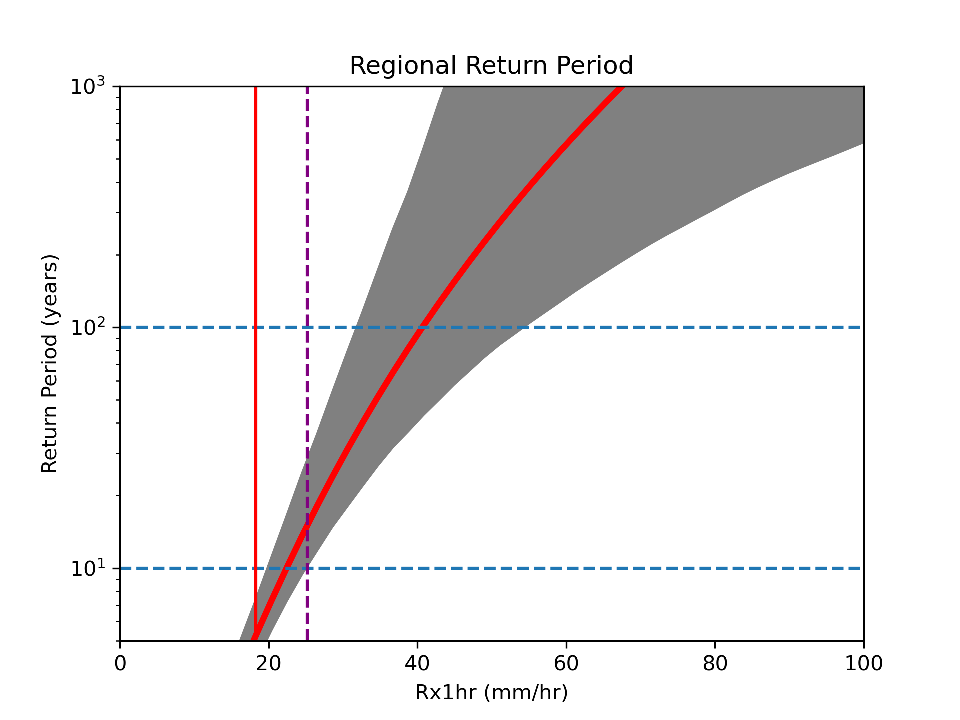
\includegraphics[width=150mm]{radarreturnplot}
    \caption[A line graph plotting the return period in years against the intensity of the event.]{
        A line graph plotting the return period in years against the intensity of the event,
        taken from fitting a GEV distribution to the event distribution.
    The dashed purple vertical line is the intensity of the Stonehaven event.
    The solid red vertical line is the actual one-hour rainfall maximum at the Stonehaven crash location.
    The grey area gives the uncertainties from a Monte Carlo bootstrap of approximately 1000 samples.
    Produced with an adaptation of the code for figure 2f of~\cite{Tett_Soon}.}
    \label{fig:radarreturnplot}
\end{figure}

It was found that the maximum hourly rainfall at the crash location was 18.2mm/hr and
    that the empirical return period for the Stonehaven event was 17 years,
    as can be seen in figure~\ref{fig:radarreturnplot}.
The intensity of the Stonehaven event,
    the 0.95 quantile of the radar grid cells having their 2020 seasonal maxima in the AM of the 12th of August,
    was found to be 25.2mm/hr.

Figure~\ref{fig:radarreturnplot} was created using the survival function of the GEV distribution fitted to the event data,
    getting the return period as the reciprocal of the probability.
This had parameters location $\mu = 10.7$, scale $\sigma = 4.26$ and shape $\xi = 0.173$.

\subsection{Model Data}\label{subsec:modelcorr}

\subsubsection{Model Correlations}

\begin{figure}[H]
    \centering
    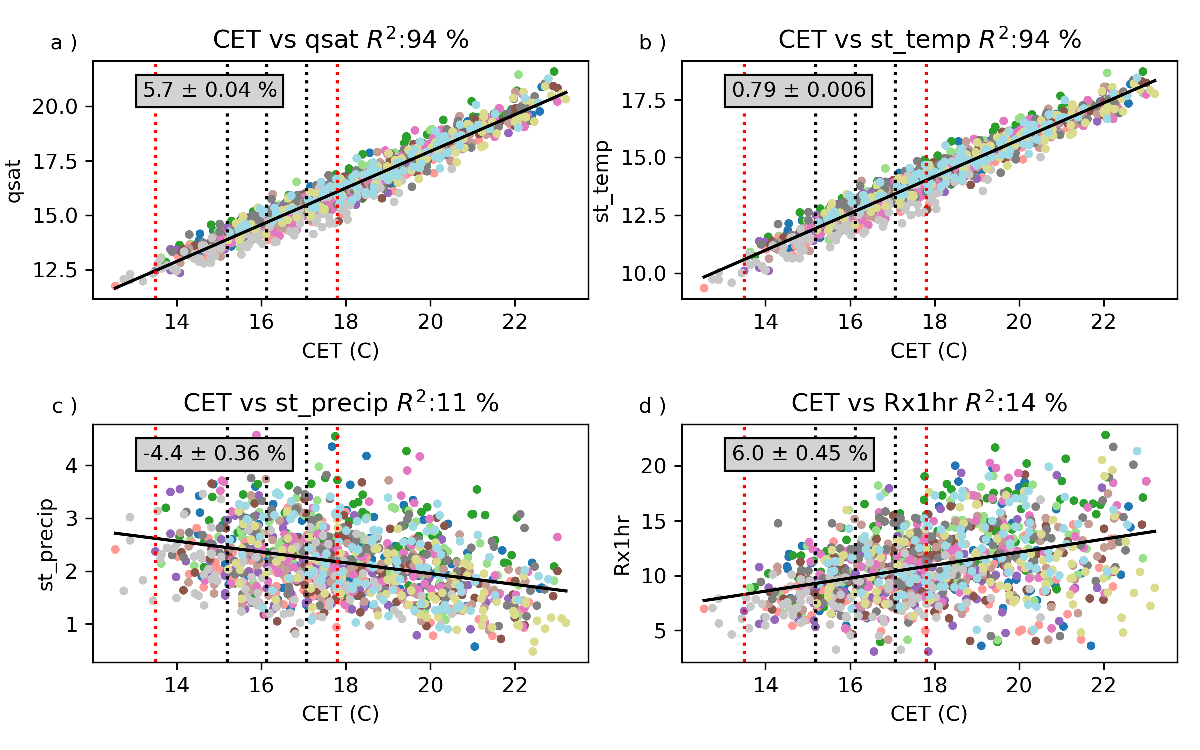
\includegraphics[width=150mm]{2cet_scatter}
    \caption[Scatter diagrams from the Convection Permitting Model.]{
        Scatter diagrams, from the Convection Permitting Model,
        for summer CET vs Stonehaven region saturated humidity (g/Kg) (a),
        Regional Temperature (b),
        Regional  Precipitation (mm/day) (c) and
        spatial median Rx1hr (mm/hr) for the region.
    The region is all points within a square of about 100x100km centered on the Stonehaven crash location.
    Colors indicate the ensemble number, black line is the best-fit regression slope.
    Text box shows best estimate and standard error in the estimated regression.
    Dotted black vertical lines show (left to right) CET summer mean for 1850--1899, 2021 and estimated CET at +2K warming.
    Title shows $R^2$ correlation coefficients for fit.
    Dotted vertical red lines show minimum and maximum CET values from 1850--2020 observations.
    Produced with an adaptation of the code for figure S1 of~\cite{Tett_Soon}}
    \label{fig:2cet_scatter}
\end{figure}

It is unsurprising that the correlations found in (a) and (b) are very similar,
    with both having $R^2$ values that round to the same number to the nearest percentage.
Some data points appear in almost identical points in both scatter diagrams.
This is evident from equation~\ref{eq:qsat}.
By differentiating at $T=18$,
    equation~\ref{eq:qsat} has Taylor series to first order of $20.5627+1.2863(T-18)$.
By substituting $T=14$ and $T=22$ into this linear approximation,
    only small errors of $0.532$ and $0.603$ are found.
This suggests that in the CET range, equation~\ref{eq:qsat} is effectively linear and so the fit onto the Stonehaven Region saturated humidity
    is a linear scaling of the fit onto the Stonehaven Region Temperature.

(b) finds that the temperature in the Stonehaven Region is expected to increase by 0.79 degrees for every increase
    in CET .
This is of interest, as CET itself is expected to increase by 0.96 per degree of climate warming~\cite{Tett_Soon},
    so the Stonehaven Region temperature is expected to increase far slower than global temperatures.

In (c),
    a negative correlation is found between the mean rain in the Stonehaven region and CET,
    suggesting that total rainfall decreases with an increase in temperature.
This contrasts with the positive correlation between the mean monthly maximum rainfall found in (d),
    which suggests that the scaling of the extreme distribution will be positive.

\subsubsection{Model GEV fit}

\begin{figure}[H]
    \centering
    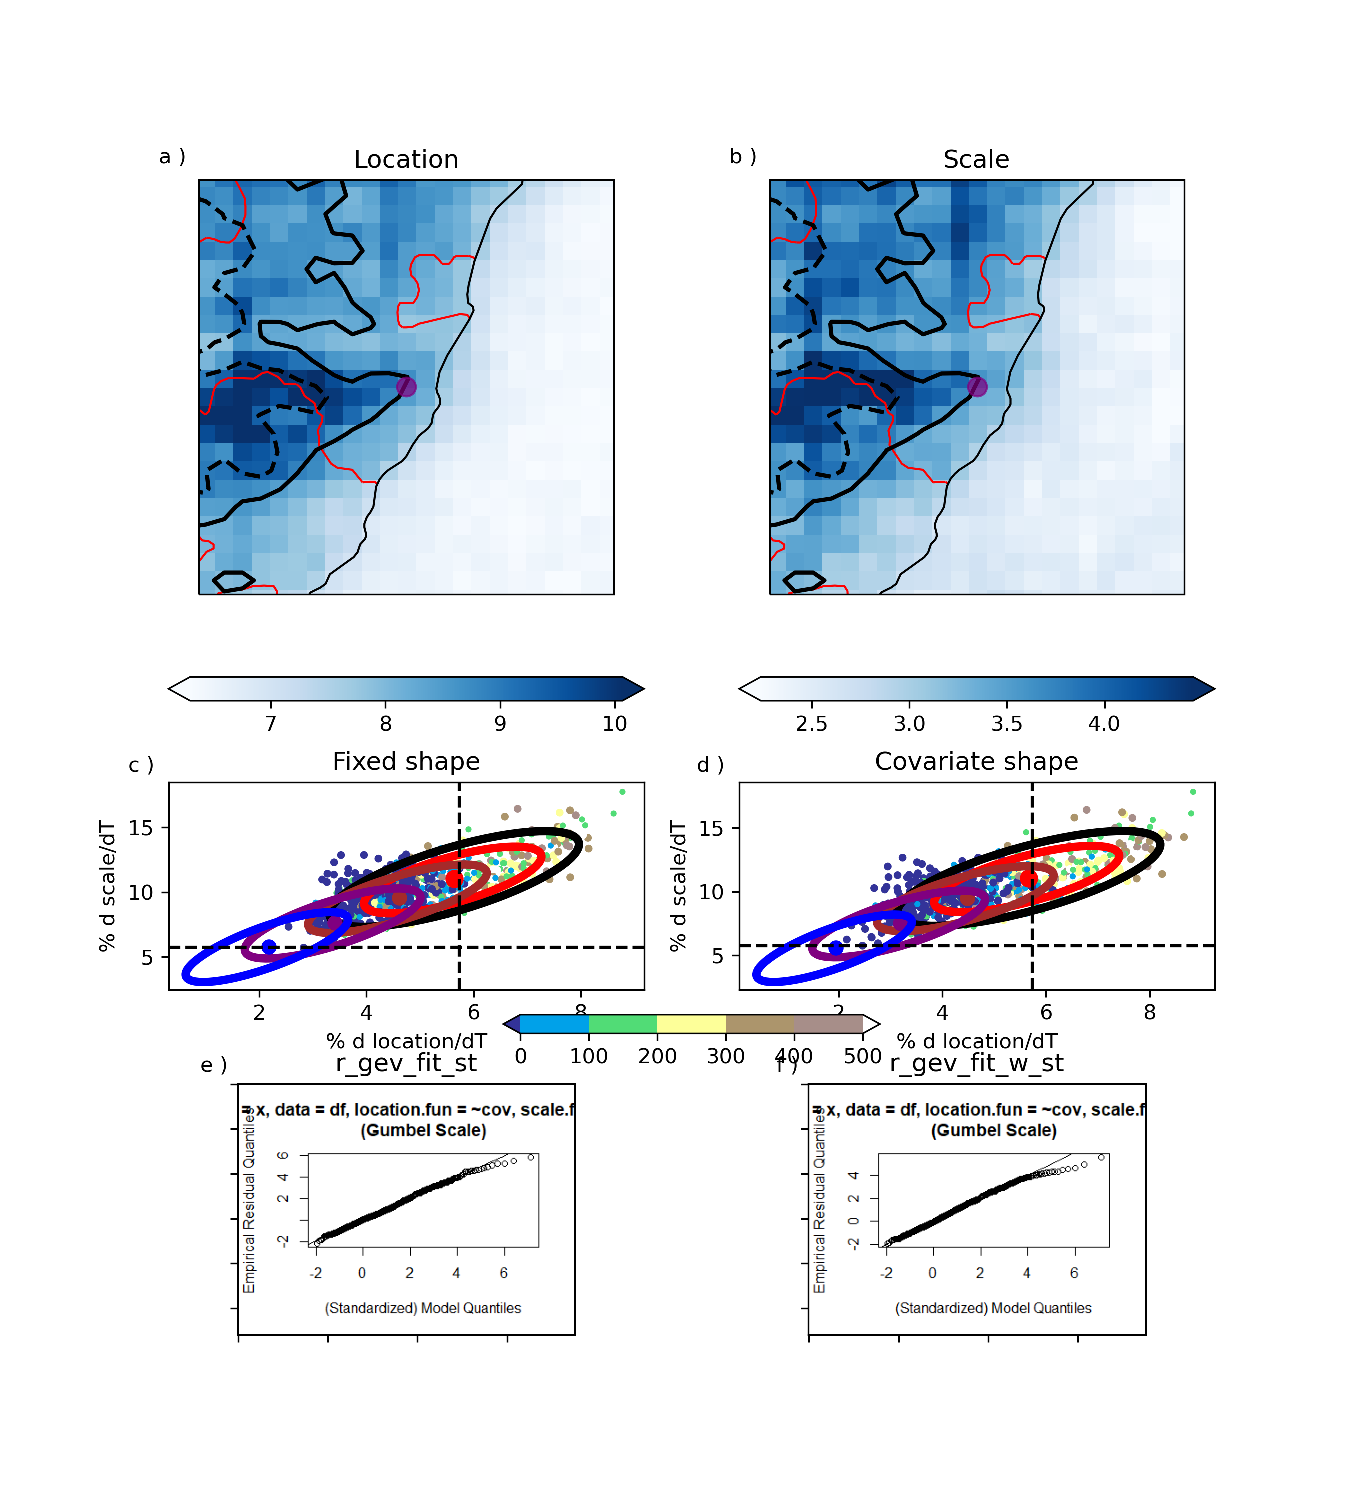
\includegraphics[width=100mm]{2cpm_gev_fit}
    \caption[a) Location parameter $\mu = \mu_0 + \overline{T_{2012-2021}}\mu_1$  for 2012--2021 CET and Rx1hr.
    b) Scale parameter $\sigma = \sigma_0 + \overline{T_{2012-2021}}\sigma_1$ for 2012--2021 CET and Rx1hr.
    c) Scatter plot of d(location)/d(CET) vs d(scale)/d(CET) as of 2012--2021 parameters.
    d) as c) but for case with shape parameter varying with CET.
    e) QQ-plot for GEV fit to CPM data using CET as a covariate at the Stonehaven Crash location.
    f) as e) but for point 25km west of the Stonehaven Crash Location.]{
        a) Location parameter $\mu = \mu_0 + \overline{T_{2012-2021}}\mu_1$  for 2012--2021 CET and Rx1hr.
    b) Scale parameter $\sigma = \sigma_0 + \overline{T_{2012-2021}}\sigma_1$ for 2012--2021 CET and Rx1hr.
    c) Scatter plot of d(location)/d(CET) vs d(scale)/d(CET) as of 2012--2021 parameters.
    Dashed lines show expected changes if changes predicted by Clausius-Clapeyron relationship.
    Dots are colored by topography.
    Large red dot shows mean over all points where height is more than 0m and less than 400m.
    Red ellipse shows 95\% uncertainty for this mean, see subsection~\ref{subsec:riskratios}.
    Other colored large dots and ellipses show similar means and uncertainty ellipses for Rx2hr (brown), Rx4hr (purple) and Rx8hr (blue).
    Black ellipse shows 95\% uncertainty for all Rx1hr points where height is less than 0m and more than 200m.
    d) as c) but for case with shape parameter varying with CET
    e) QQ-plot for GEV fit to CPM data using CET as a covariate at the Stonehaven Crash location.
    f) as e) but for point 25km west of the Stonehaven Crash Location.
    Produced with an adaptation of the code for figure S3 of~\cite{Tett_Soon}}
    \label{fig:2cpm_gev_fit}
\end{figure}

The thin, thick and dashed lines on (a) and (b) represent 0m, 200m and 400m contours respectively.
These charts show that the rainfall is expected to be greater over higher areas,
    with the extreme rainfall distribution having both greater location and scale parameters,
    which are a factor of approximately 1.5x greater over 400m than they are between 0m and 200m.
The rainfall over the sea is extremely low.
This should be disregarded for reasons given in subsection~\ref{subsec:preprocess}

The colours of the dots in (c) show that the increase of both the shape and scale parameters with CET
    increases with height,
    although, as a proportion of the base parameter, there is no evidence for additional scaling with height,
    as, from (a) and (b), higher grid cells have higher base values for the parameters.
The confidence ellipses show that there is far greater uncertainty about the increase in the location parameter
    than the scale parameter.
The similarity of (b) and (c) suggest that fitting the shape parameter as to the covariate does not have
    a significant effect on the fit of the other two parameters to the covariate.
Table~\ref{tab:CCtable} gives the location of the red, brown, purple and blue dots relative to the
    dashed lines representing Clausius-Clapeyron scaling.

(e) shows that the quantiles for the GEV fit are similar at the Stonehaven Crash location,
    while (f) is taken from a point near the 400m contour.
At this point, the GEV fit breaks down at the top end,
    with the GEV fit expecting values far greater than those provided by the CPM model it is fit to.

\begin{table}[H]
    \centering
    \begin{tabular}{c c c c c}
        Covariate\textbackslash Data & Rx1h & Rx2h & Rx4h & Rx8h \\
        None &7498&6533&5341&4130 \\
        CET &7433&6482&5305&4109 \\
        CET w/ Shape &7434&6483&5305&4109 \\
        CPM Region &7402&6457&5287&4097 \\
        CPM Region w/ Shape &7403&6458&5287&4097 \\
        Stonehaven Region &7402&6457&5287&4098 \\
        Stonehaven Region w/ Shape &7403&6458&5288&4098 \\
        Stonehaven Humidity &7405&6459&5289&4099 \\
        Stonehaven Humidity w/ Shape &7406&6460&5290&4100 \\
    \end{tabular}
    \caption[AIC for maximum summer rainfall]{
        AIC for maximum summer 1, 2, 4 and 8 hourly summer maximum rainfall
        above 0m and below 400m in the Stonehaven Region (+/- 0.5 degrees of the Stonehaven Crash location)
        GEV fits with different covariates.
    The covariates are CET, the average temperature in the CPM region (UK),
    the average temperature in the Stonehaven Region and
    the Saturation Humidity in the Stonehaven Region}
    \label{tab:AICtable}
\end{table}

The values of AIC for different rain intervals are not directly comparable,
    as the fit is to different datasets.
For all covariates,
    it is found that fitting the shape to the covariate had no significant effect on the goodness of the GEV fit.
For the 1 hour maxima,
    fitting the GEV with the CPM Region temperature, Stonehaven Region Temperature and Stonehaven Region Humidity gave almost equally good fits.
It was expected that the fit to the Stonehaven Region Temperature and Humidity would be similar for
    reasons given in the discussion of~\ref{fig:2cet_scatter},
    although Humidity does perform slightly worse as a covariate.
Having no covariate provides a worse fit for the data.

The probability of information loss formula, equation~\ref{eq:AIC_Info},
    can be applied to the AIC values in table~\ref{tab:AICtable} for the one hour maximum model rainfall.
This finds that a fit to CET is of order $10^{-7}$ times as probable to be a better fit than to another covariate,
    and that a fit to no covariate is of order $10^{-21}$ times as probable to be a better fit than to a covariate other than CET .

\begin{table}[H]
    \centering
    \begin{tabular}{c c c}
        Dataset\textbackslash Parameter  & Location $\mu$ & Scale $\sigma$ \\
        Rx1hr &0.98&1.92 \\
        Rx2hr &0.80&1.67 \\
        Rx4hr &0.59&1.33 \\
        Rx8hr &0.38&1.01 \\
    \end{tabular}
    \caption[Ratio of mean parameter scalings to Clausius-Clapeyron scaling.]{
        Ratio of mean parameter scalings to Clausius-Clapeyron scaling, $\left( \frac{\alpha_1}{\alpha_0} \right) / \left( \frac{H_1}{H_0} \right)$,
        for parameter $\alpha$ in the GEV fit to CET and saturated humidity $H$ in a linear fit to CET,
        where the shape parameter is fixed for the fit.
        Subscript $0$ is the value in the average summer CET of 2012--2021,
            subscript $1$ is the increase for every one degree increase of CET.
    Clausius-Clapeyron scaling is 5.73\%.}
    \label{tab:CCtable}
\end{table}

The scaling of all the parameters in table~\ref{tab:CCtable} are positive,
    as would be expected from figure~\ref{fig:2cet_scatter} (d),
    which shows that the maximum rainfall extrema increase with CET .
For the one-hour rainfall maxima,
    the location is scaled almost exactly as would be expected with Clausius-Clapeyron,
    shown by the red dot in figure~\ref{fig:2cpm_gev_fit} (c) being almost exactly on the vertical dashed line,
    while the scale parameter is scaled almost double that expected by Clausius-Clapeyron.
Figure~\ref{fig:2cet_scatter} (a) and (d) also suggest this pattern,
    as the both the saturated humidity and 1 hour maximum rainfall increase by around 6 (ignoring units)
    per degree increase in CET, while saturated humidity takes a value at around 15 for a typical CET,
    with Rx1hr taking a value of 10 and so having a larger proportional increase per degree of warming.
This agrees with the IPCC working group 1 assessment~\cite{IPCC_2021},
    finding that sub-daily extreme precipitation scales between one and two times that of Clausius-Clapeyron.

As the time period of the extrema increases,
    the scaling of the parameters decrease.
Figure~\ref{fig:2cet_scatter} (c) suggests that this is to be expected,
    as non-extreme rainfall in the Stonehaven decreases with CET and so by averaging over a longer time period,
    the maximum rainfall exhibits behaviour more similar to average rainfall.
However, this finding is surprising in a wider context,
    as the IPCC assessment~\cite{IPCC_2021} states that the scaling in excess of Clausius-Clapeyron should apply to all sub-daily precipitation extremes,
    and all of the extrema given in this report are sub-daily.

The scale parameter $\sigma$ scales by more per increase in CET than the location parameter $\mu$.
The effect of this is that the modelled maximum rainfall in a typical year does not increase by a large amount,
    but for more extreme years, those with higher return periods,
    the maximum rainfall increases by a larger amount with CET than would be expected with Clausius-Clapeyron.

Where the shape parameter is fit as a covariate,
    the change in the shape parameter per degree increase of CET $\xi_1$ is
    0.004, 0.055, 0.128 and 0.252 for the maximum summer model rainfall in
    1 hour, 2 hour, 4 hour and 8 hour time periods respectively.
The risk ratios will be calculated using the one-hour maximum,
    so the covariate fit of the shape parameter is expected to have little effect on these.

\subsection{Risk Ratios}\label{subsec:riskratio}

\begin{figure}[H]
    \centering
    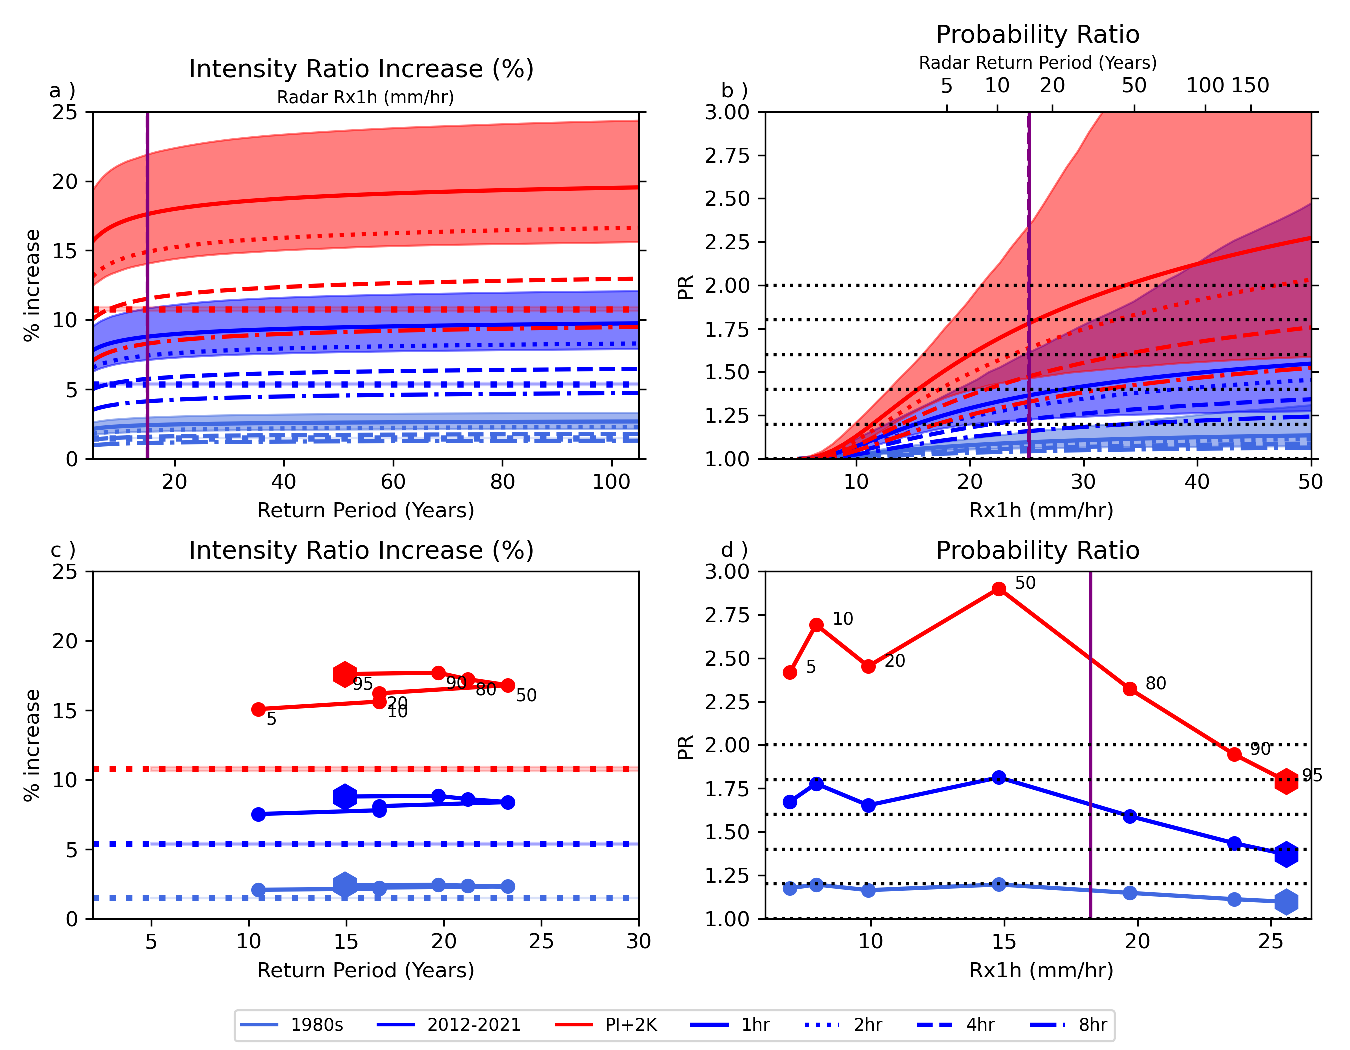
\includegraphics[width=\linewidth]{2probradarcpm}
    \caption[Intensity ratio (\%) as a function of the return period (a,c) and
    probability ratio as a function of regional Rx1hr (b, d).
    ]{
        Intensity ratio (\%) as a function of the return period (a) and
    probability ratio as a function of regional Rx1hr (b).
    The best estimate (line) and 5--95\% uncertainty range (shading) are shown.
    Horizontal dotted lines in a) show expected intensity change if extremes scale with Clausius-Clapeyron.
    The top axis in a and b shows the equivalent rainfall and return period estimated from the radar rainfall data while
    vertical purple line shows the regional rainfall maximum for 2020.
    Dotted, dashed and dot-dashed lines in a and b show results when scaling estimated from simulated 2, 4 and 8 hourly summer maxima (Rx2hr, Rx4hr and Rx8hr).
    c) Intensity ratio (\%) as a function of return period for best estimates using different quantiles (labels on PI+2K line) to define regional extreme.
    Hexagon markers show 95\% quantile used in a and b.
    d) As c) but for probability ratio as a function of Rx1hr.
    Vertical purple line shows Stonehaven Crash Rx1hr for 2020-08-12.
    Note these are different from the regional 95\% quantiles shown in (a) and (b).
    Produced with an adaptation of the code for figure 3 of~\cite{Tett_Soon}.}
    \label{fig:2probradarcpm}
\end{figure}

Figure~\ref{fig:2probradarcpm} (a) shows that the intensity ratio decreases when fitted to model extrema over longer intervals,
    only being sub-Clausius-Clapeyron when the event distribution is scaled like the average over 8 hour model maxima;
(b) shows the same decreasing in risk ratios for scaling like longer-interval model maxima.
This is to be expected from the data in table~\ref{tab:CCtable},
    as it is known that maxima over longer periods give a lower scaling.

The intensity and probability ratios in (a) and (b) increase with return period and event intensity.
This is as short return period/low intensity events are in the bulk of the GEV distribution
    where the location parameter $\mu$ dominates, while long return period/high intensity events are in the tail of
    the distribution, where scale parameter $\sigma$ dominates behaviour.
The ratio of the intensity ratio to the Clausius-Clapeyron scaling, given by the dotted lines,
    tends to the scaling of $\sigma$ relative to Clausius-Clapeyron,
    given in table~\ref{tab:CCtable}, multiplied by the CET difference from Pre-Industrial as the return period tends to infinity.
This increase is from the scaling of $\mu$ relative to Clausius-Clapeyron multiplied by CET difference at a return period of
    $\left( 1- e^{-1} \right)^{-1} \approx 1.6$, obtained by inverting equation~\ref{eq:gevreturn}.

(c) Shows that there is little difference in the intensity ratio by defining the Stonehaven Event by a different
    quantile, with all the intensity ratios super-Clausius-Clapeyron and within the confidence interval
    for the intensity ratio of the 0.95 quantile visible in (a).
(c) also shows that the most unusual extrema of the Stonehaven Event were at the 0.5 and 0.8 quantiles,
    both being rarer than 1-in-20 year events, as opposed to the 0.95 quantile definition used in the
    rest of the analysis, which was a 1-in-17 year event.

(d) shows that the probability ratio decreases with the quantile chosen for event definition from the 0.5 quantile onwards,
    going from the 0.5 quantile having a probability ratio of almost 3,
    while the 0.95 quantile has a probability ratio of around 1.8, visible in from the solid red line (b).
Additionally, (d) shows that the Stonehaven Crash location had maximum rainfall between the 0.5 and 0.8 quantiles of the Stonehaven Event,
    not at the 0.95 quantile.

\begin{figure}[H]
    \centering
    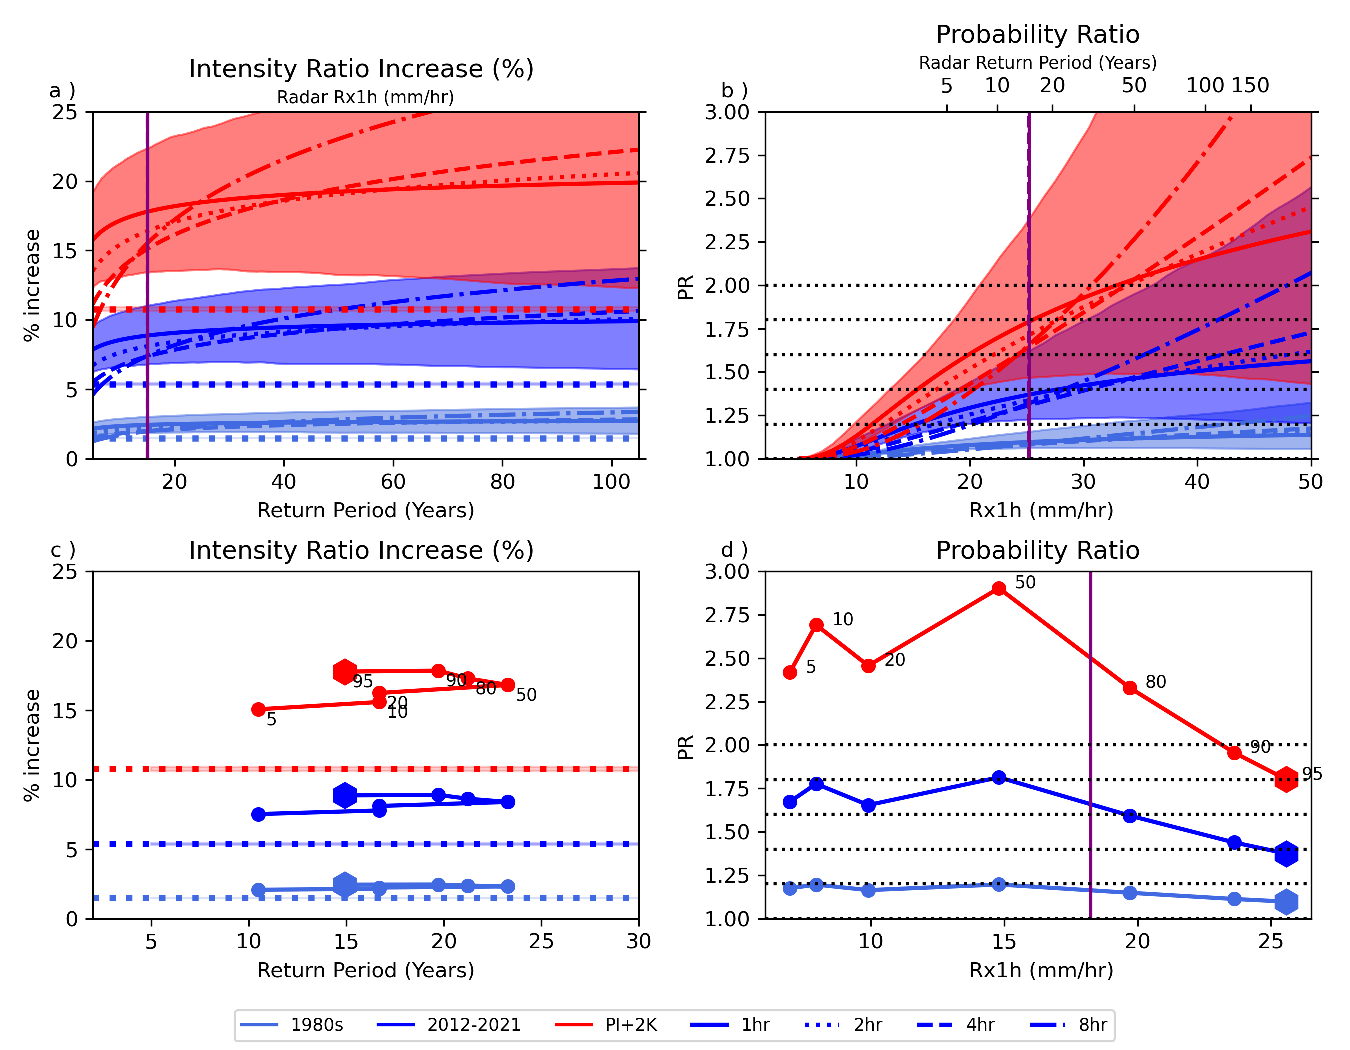
\includegraphics[width=\linewidth]{2probradarcpmshape}
    \caption[Figure~\ref{fig:2probradarcpm} with a covariate fit shape.]{
        As for figure~\ref{fig:2probradarcpm},
    with the shape parameter also allowed to vary with CET.}
    \label{fig:2probradarcpmshape}
\end{figure}

Figure~\ref{fig:2probradarcpmshape} (c) and (d) show no difference from (c) and (d) of~\ref{fig:2probradarcpm}.
This allows it to be concluded that fitting the shape parameter of the Rx1hr model data as to a CET covariate has
    no impact on the intensity or probability ratio,
    independent of the choice of quantile used to define the intensity of an Event.

(a) and (b) show the same effects as (a) and (b) of~\ref{fig:2probradarcpm} at the return period and intensity
    of the Stonehaven Event,
    with the ratios decreasing with the time interval of model maxima fit to,
    except with broader (weaker) confidence intervals.
However,
    for events with a return period of more than 25 years or an intensity of more than 30mm/hr,
    the effect starts to reverse,
    with the fit to the 8-hour model maxima giving the largest ratios.
The pattern in (a) and (b) of figure~\ref{fig:2probradarcpm} is completely reversed by return periods of
    more than 45 years or intensities of more than 35mm/hr,
    with both the intensity and probability ratios increasing with the time interval of the maxima.
This occurs as the increase in the shape parameter with CET for the larger model maxima time intervals causes the
    distributions scaled to these to also have a larger shape parameter,
    and so a longer tail and greater likelihood of more extreme events.

\begin{table}[H]
   \centering
    \begin{tabular}{c c c}
        Time Period & Intensity Ratio (\%) & 5--95\% Confidence Interval (\%) \\
        1980s & 2 & 2--3 \\
        2012--2021 & 9 & 7--11 \\
        PI+2K & 18 & 14--22 \\
        With varying shape: && \\
        1980s & 2 & 2--3 \\
        2012--2021 & 9 & 7--11 \\
        PI+2K & 18 & 13--22 \\
    \end{tabular}
    \caption[A table with the intensity ratios.]{
        A table with the intensity ratios $I_1/I_0$ for three different time periods,
        both with and without a covariate shape parameter.
    $I_1$ is the intensity of the event in the Time Period.
    $I_0$ is the intensity of the event Pre-Industrial (1850-1899).}
    \label{tab:irtable}
\end{table}

\begin{table}[H]
   \centering
    \begin{tabular}{c c c}
        Time Period & Probability Ratio & 5--95\% confidence interval \\
        1980s & 1.10 & 1.06--1.15 \\
        2012--2021 & 1.37 & 1.22--1.61 \\
        PI+2K & 1.78 & 1.46--2.34 \\
        With varying shape: && \\
        1980s & 1.10 & 1.06--1.15 \\
        2012--2021 & 1.37 & 1.23--1.62 \\
        PI+2K & 1.79 & 1.47--2.38 \\
    \end{tabular}
    \caption[A table with the probability ratios.]{A table with the probability ratios $p_1/p_0$ with confidence intervals for three different time periods,
        both with and without a covariate shape parameter.
    $p_1$ is the probability of the event in the Time Period.
    $p_0$ is the probability of the event Pre-Industrial (1850-1899).}
    \label{tab:prtable}
\end{table}

Tables~\ref{tab:irtable} and~\ref{tab:prtable} show that,
    as expected from the parameters scaling positively with CET,
    the both the intensity and probability of the event increase for later time periods,
    when CET is greater.
The ratios represent the intersections of the solid lines with the purple vertical lines in (a) and (b)
    of figures~\ref{fig:2probradarcpm} and~\ref{fig:2probradarcpmshape},
    with the confidence intervals representing the intersection of the shaded areas with the purple vertical line.

Both the ratios and confidence intervals show either no or very little difference from fitting the shape as a covariate.

By assuming that the Stonehaven event occurred in a month of typical CET to the 2012--2012 time period,
    the change in the intensity from 25.2mm/hr and return period of 17 years can be calculated.
Pre-industrial,
    the event would have had an intensity of 23.1 (CI: 22.7--23.6) mm/hr and a return period
    of 23.3 (20.9--27.5) years.
In a world 2K warmer than industrial,
     the event would have had an intensity of 27.3 (26.8--27.7) mm/hr and a return period
    of 13.1 (11.7--14.2) years.

\begin{table}[H]
    \centering
    \begin{tabular}{c c c}
        Time Period\textbackslash Parameter & Location $\mu$ & Scale $\sigma$ \\
        PI & 10.2 & 3.90 \\
        1980s & 10.4 & 4.02 \\
        2012--2021 & 10.8 & 4.34 \\
        PI+2K & 11.3 & 4.79
    \end{tabular}
    \caption[Parameters of the GEV distribution for the intensity an event.]{
        A table showing the parameters of the GEV distribution for the intensity an event defined in subsection~\ref{subsec:radarprocess} after
        applying the scaling of the location $\mu$ and scale $\sigma$ parameters to the temperatures of different time periods.}
    \label{tab:0.95params}
\end{table}

The data in table~\ref{tab:0.95params} does not have a the shape scaled from the CET covariate,
    using the fixed shape parameter $\xi = 0.173$ from the empirical fit.
The shape parameter is in the $0.174$--$0.172$ range for all three fits with covariate shape,
    so it effectively duplicates the parameters here.

Note that as the shape parameter is positive,
    this fit suggests that, with an infinite return period, there is no limit on the maximum hourly rainfall.
While is clearly unphysical, the positive shape parameter gives a minimum possible value of event intensity in a given summer as
    -12.3, -12.8, -14.3 and -16.3 mm/hr for the PI, the 1980s, 2012--2021 and PI+2K Time Periods respectively.
This is clearly also unphysical,
    as rainfall cannot be negative,
    showing that the distribution is inappropriate in the infinite limit in either direction.
However,
    the inference is still valid when interpolating in higher probability dense areas of the distribution,
    where the mean event intensity is 13.2, 13.5, 14.2 and 15.0 mm/hr and
    the median event intensity is 11.7, 11.9, 12.4 and 13.1 mm/hr for
    events in the PI, the 1980s, 2012--2021 and PI+2K Time Periods respectively.

\begin{figure}[H]
    \centering
    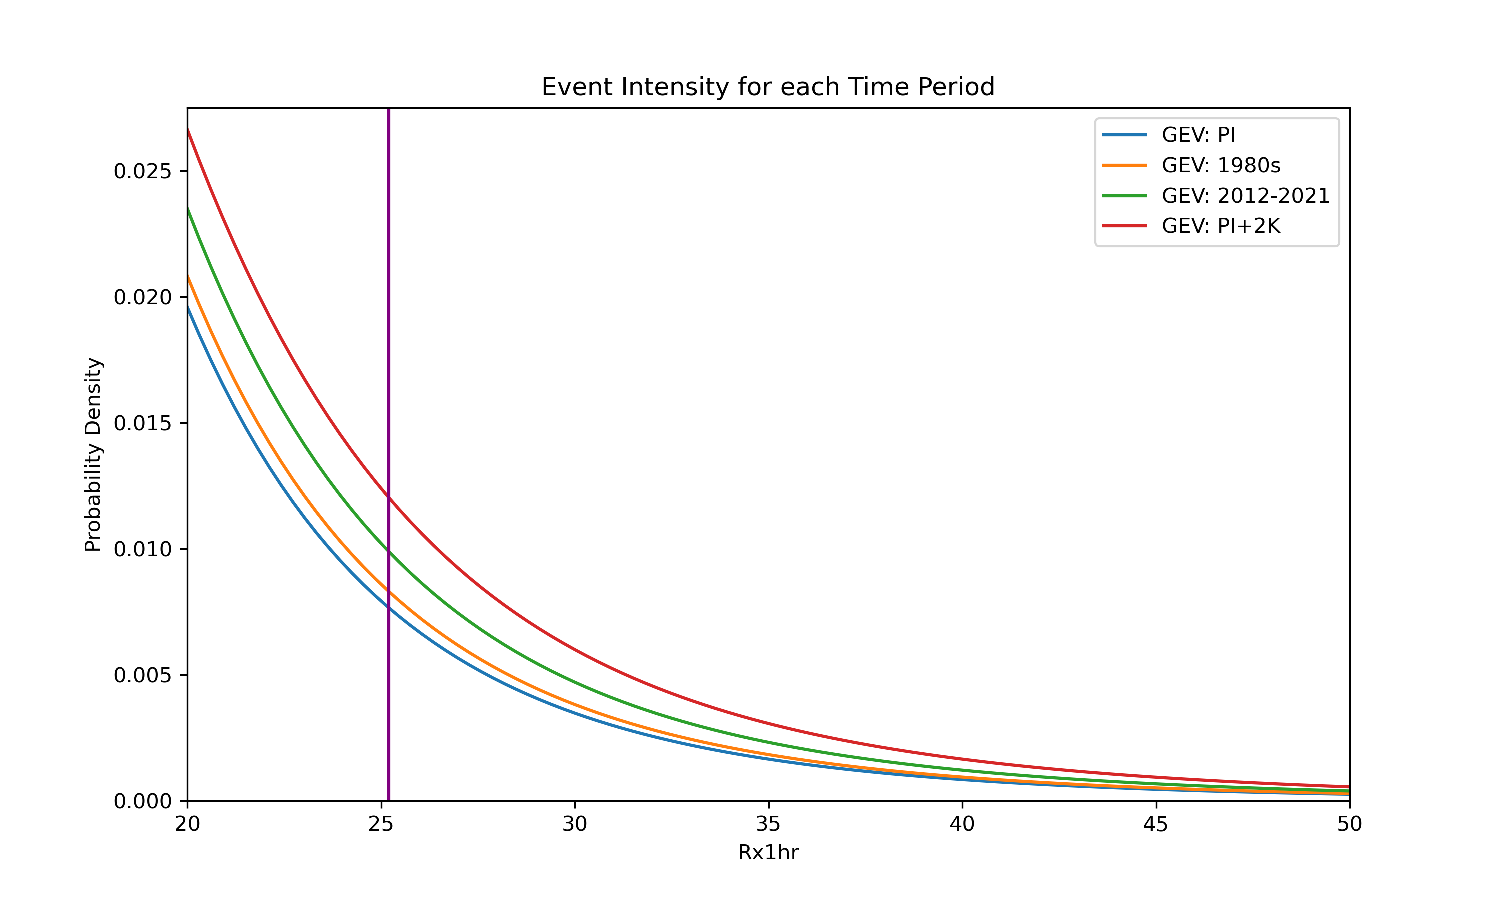
\includegraphics[width=150mm]{scaledgevdists}
    \caption[PDFs of the GEV distributions.]{
        A line chart of the Probability Density Functions of the GEV distributions with parameters given in table~\ref{tab:0.95params},
        with a shape parameter $\xi = 0.173$.
    The Time periods are Pre-Industrial (PI), the 1980s, 2012--2021
    X-axis gives the 0.95 quantile of the maximum summer rainfall by grid cell in mm/hr,
        Y-axis gives the probability density in probability/(mm/hr).
    Vertical purple line is the intensity of the Stonehaven Event.}
    \label{fig:scaledgevdists}
\end{figure}

Figure~\ref{fig:scaledgevdists} illustrates the probability ratios in the top half of table~\ref{tab:prtable}.
$p_0$ is the area to the right of the purple line between 0 and the blue curve,
    while $p_1$ is the area to the right of the purple line between 0 and the yellow, green and red curves for
    the 1980s, 2012--2021 and a world 2K warmer than pre-industrial respectively.


\section{Discussion}\label{sec:discussion}

\begin{comment}
This section should give a picture of what you have taken out of your
project and how you can put it into context.

This section should summarise the results obtained, detail conclusions
reached, suggest future work, and changes that you would make if you
repeated the project.
\end{comment}

\subsection{Model Resolution}\label{subsec:dismodeldef}

One difference between the measurement of distributions in the model and the empirical distribution is that the radar data is on 5x5km grid,
    while the model distributions are fit from model rainfall on a 4.4x4.4km grid constructed from the original 2.2x2.2km model resolution.
Kendon, Fischer and Short~\cite{Kendon_Fischer_Short_2023}, also using 100 year long 2.2km resolution climate models,
    found that a fine resolution gave a 4x increase in the risk of rainfall exceeding 20mm/hr,
    while a coarser resolution gave only a 2.6x increase.

The model analysis and risk ratio analysis described in section~\ref{sec:model} was repeated,
    except with the model either having no pre-processing other than the height mask,
    maintaining the original 2.2km resolution,
    or with the model being coarsened to take the average of sets of 3x3 grid cells,
    giving a 6.6km resolution.

\subsubsection{Model Fits}

\begin{figure}[H]
    \centering
    \begin{subfigure}{0.48\textwidth}
        \centering
        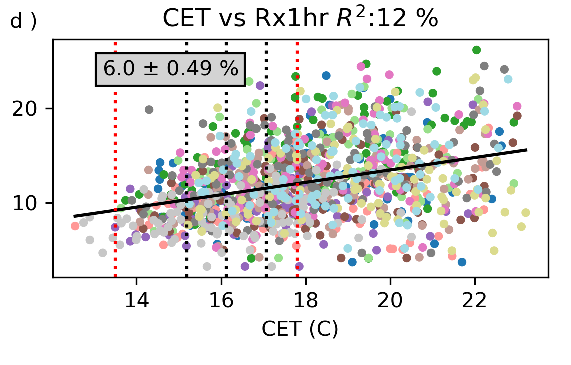
\includegraphics[width=\linewidth]{1cet_scatter}
    \end{subfigure}
    \hfill
    \begin{subfigure}{0.48\textwidth}
        \centering
        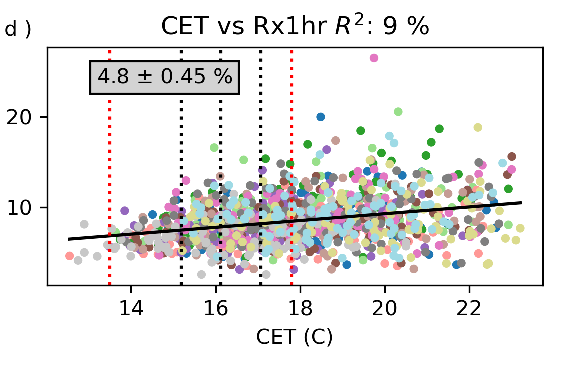
\includegraphics[width=\linewidth]{3cet_scatter}
    \end{subfigure}
    \caption[Figure~\ref{fig:2cet_scatter} with 2.2km and 6.6km fits.]{
        Figure~\ref{fig:2cet_scatter} (d), with the 1 hour model rainfall maxima of the 2.2km resolution (left) and 6.6km resolution (right) models.}
    \label{fig:13cet_scatter}
\end{figure}

Figure~\ref{fig:2cet_scatter} (d) shows that
    one hour rainfall maxima for the 4.4km model increases by 6.0mm/hr per degree increase in CET,
    matching the increase in the 2.2km model here,
    while the 6.6km model gives a slower increase in rainfall maxima per degree increase in CET .
However, at a typical CET of 16 degrees Celsius,
    the maximum rainfall in the 6.6km is approximately one fifth smaller than in the other models,
    suggesting that the scaling of the maximum rainfall with CET will be similar.
The 4.4km model is best correlated with CET, with an $R^2$ value of 14\% being greater than either of the alternative models.

\begin{figure}[H]
    \centering
    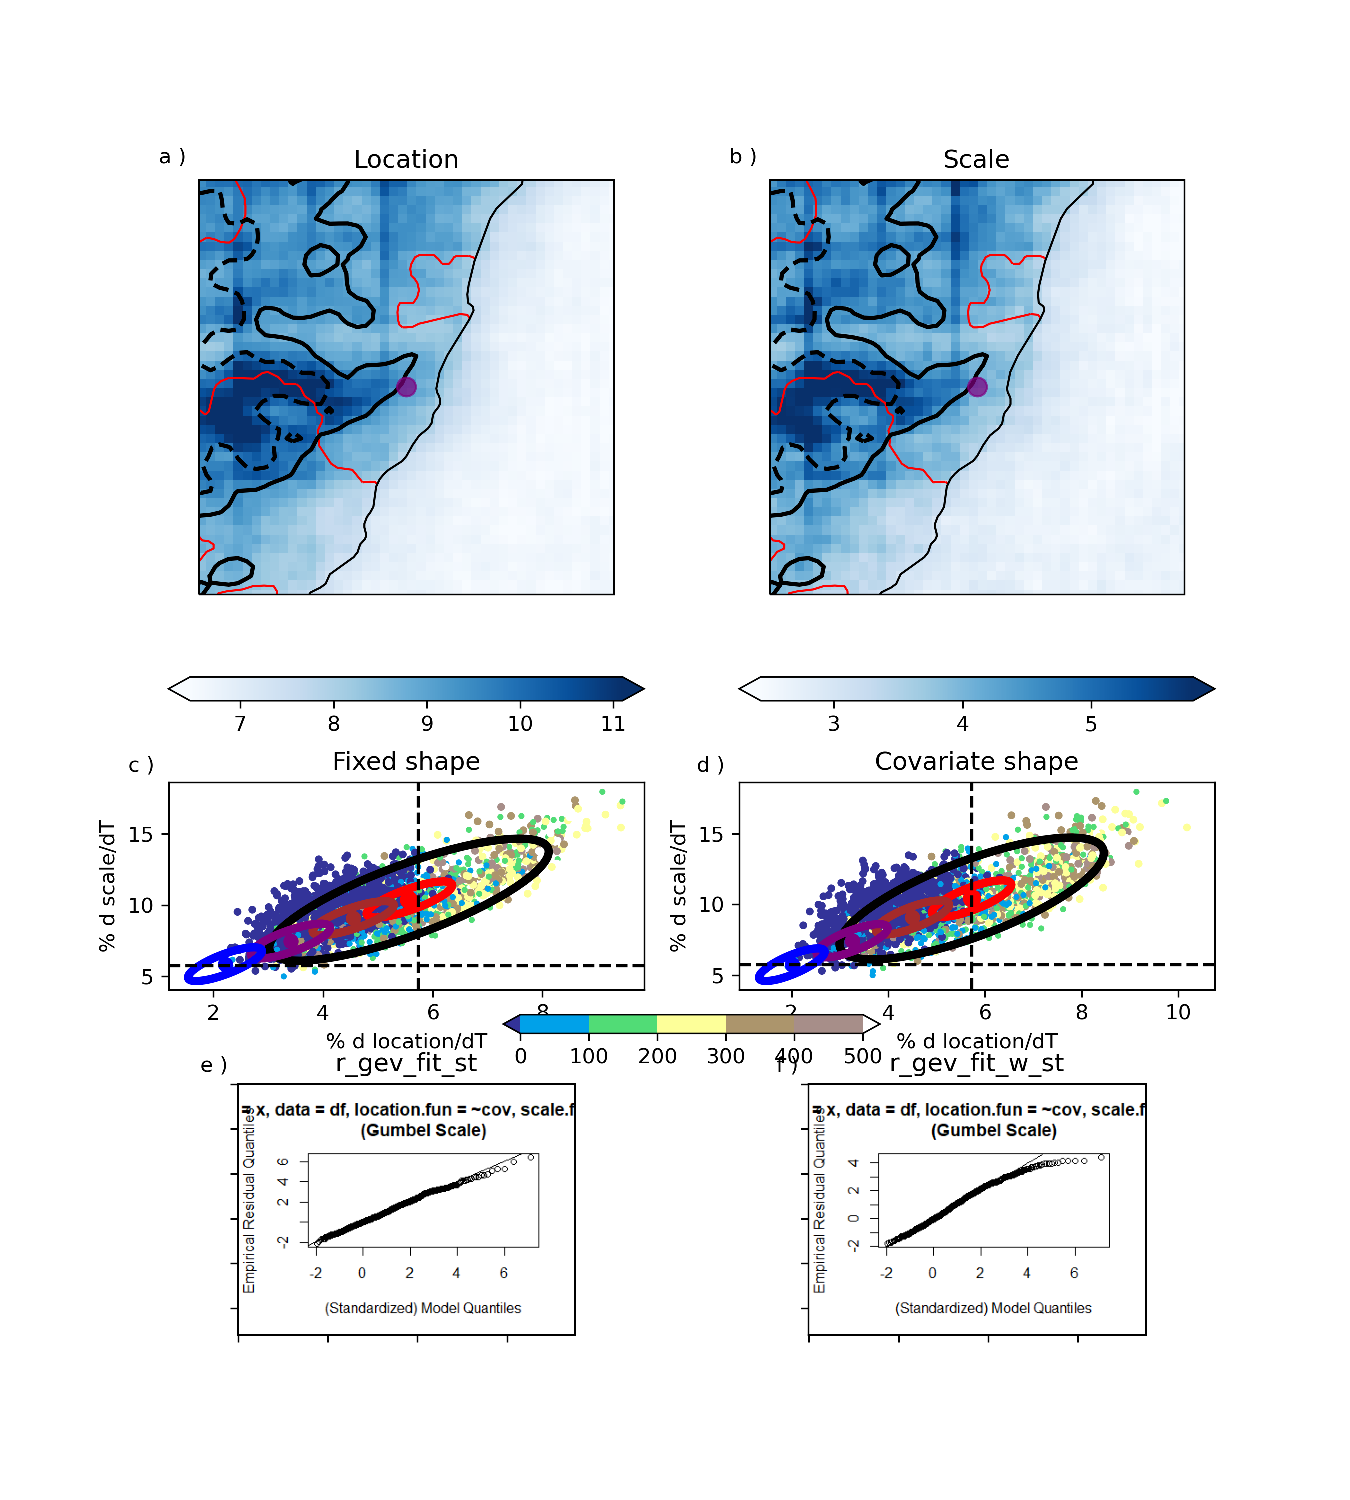
\includegraphics[width=150mm]{1cpm_gev_fit}
    \caption{Figure~\ref{fig:2cpm_gev_fit}, with the 2.2km resolution model}
    \label{fig:1cpm_gev_fit}
\end{figure}

(a) and (b) of figure~\ref{fig:1cpm_gev_fit} appear very similar to
    (a) and (b) of figure~\ref{fig:2cpm_gev_fit}.
However, note that the scale bar is different in each figure,
    with the values being approximately 1.5x greater in the model without coarsening.
This is as the grid cells take maximum summer rainfall values at different times,
    resulting in coarsening before taking the maxima giving results lower than taking the maxima and coarsening after.

(c) and (d) are also very similar between figures~\ref{fig:1cpm_gev_fit} and~\ref{fig:2cpm_gev_fit},
    with the primary difference between them being the smaller (stronger) confidence intervals in the more fine models.
This is to be expected, as there are more data points to be sampled.

\subsubsection{Risk Ratios}

\begin{figure}[H]
    \centering
    \begin{subfigure}{0.48\textwidth}
        \centering
        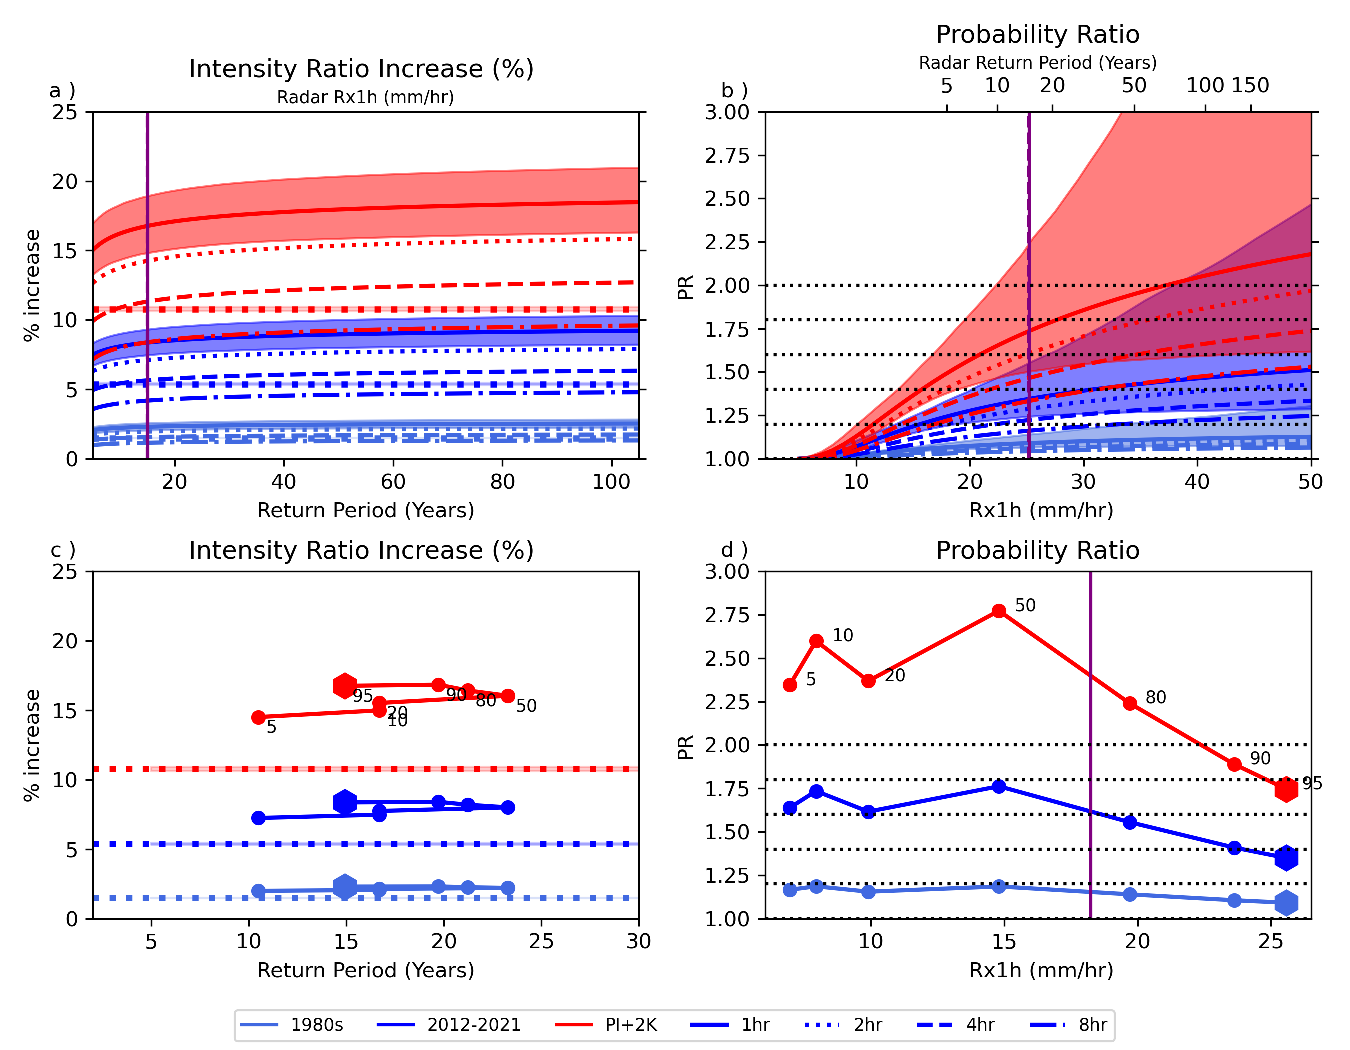
\includegraphics[width=\linewidth]{1probradarcpm}
    \end{subfigure}
    \hfill
    \begin{subfigure}{0.48\textwidth}
        \centering
        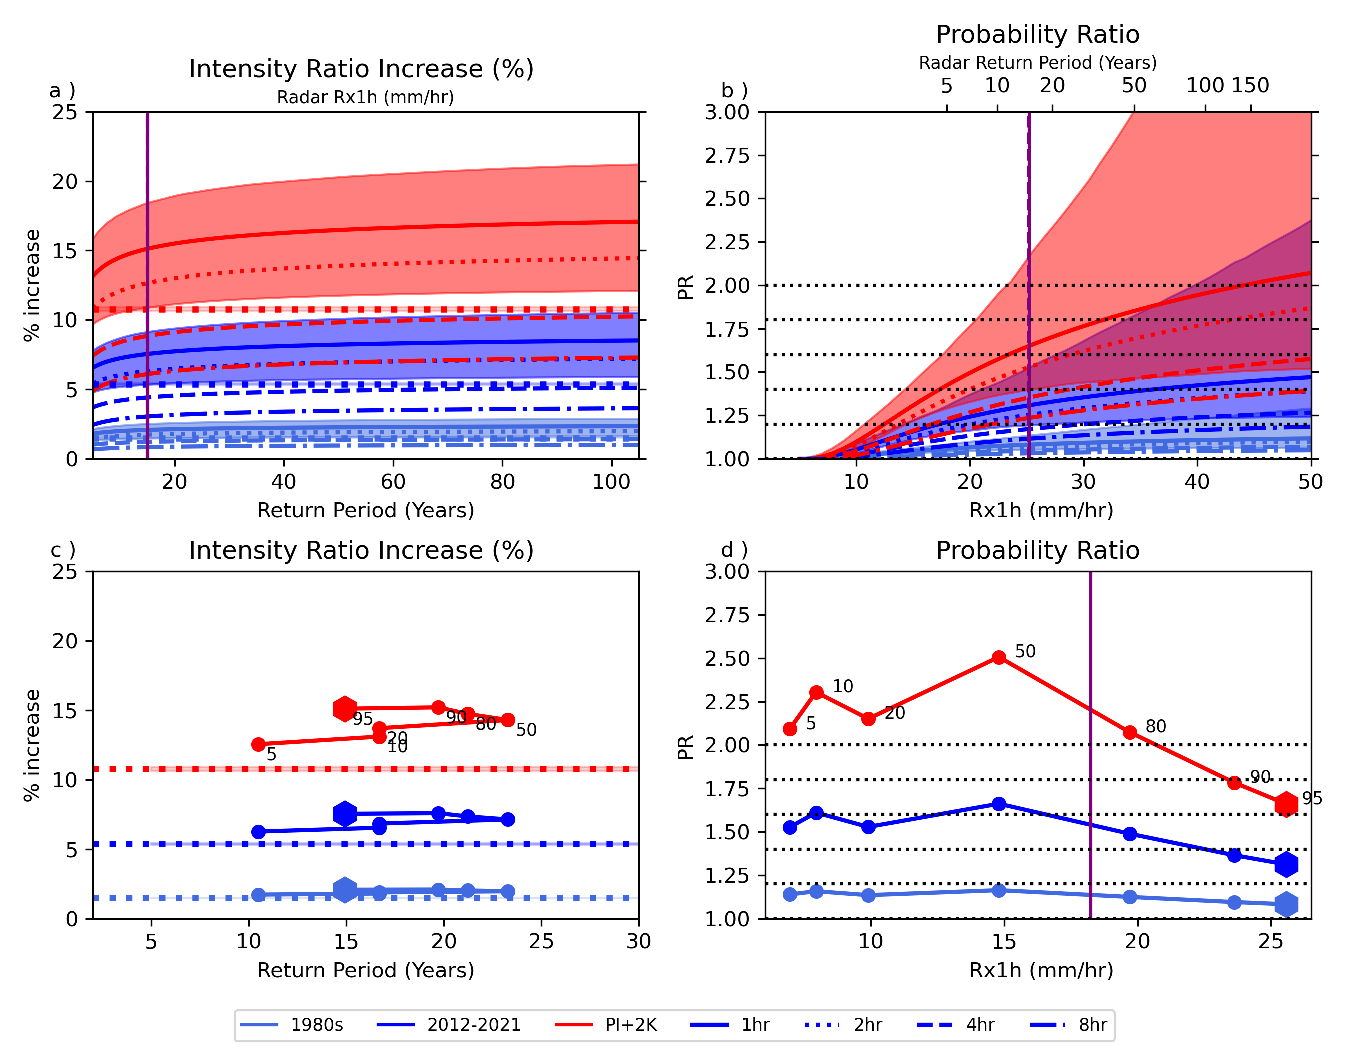
\includegraphics[width=\linewidth]{3probradarcpm}
    \end{subfigure}
    \begin{subfigure}{0.48\textwidth}
        \centering
        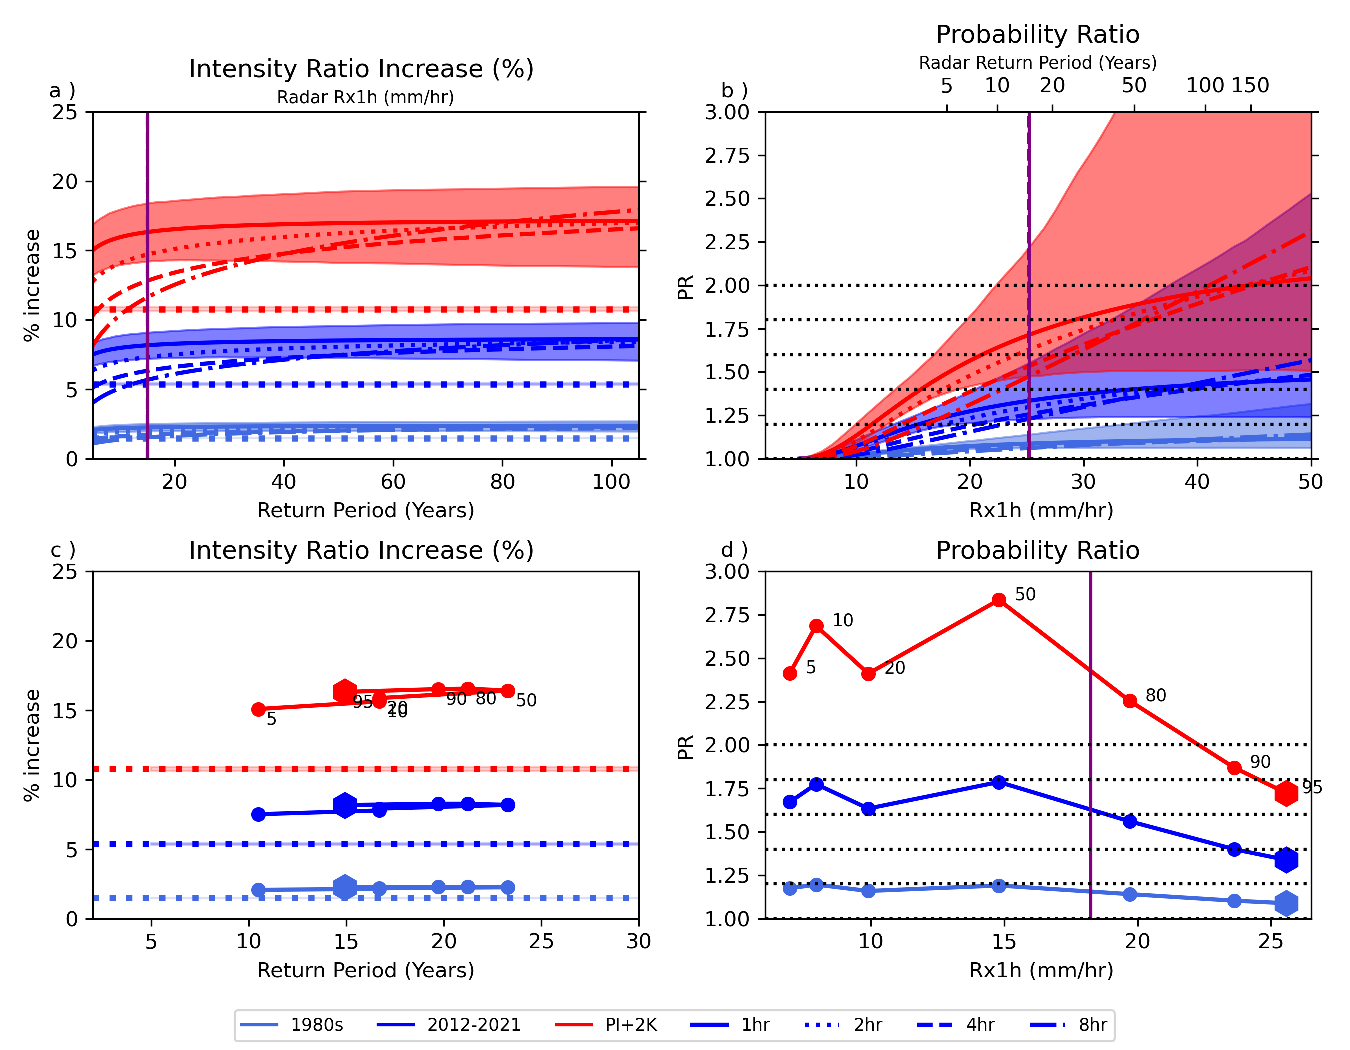
\includegraphics[width=\linewidth]{1probradarcpmshape}
    \end{subfigure}
    \hfill
    \begin{subfigure}{0.48\textwidth}
        \centering
        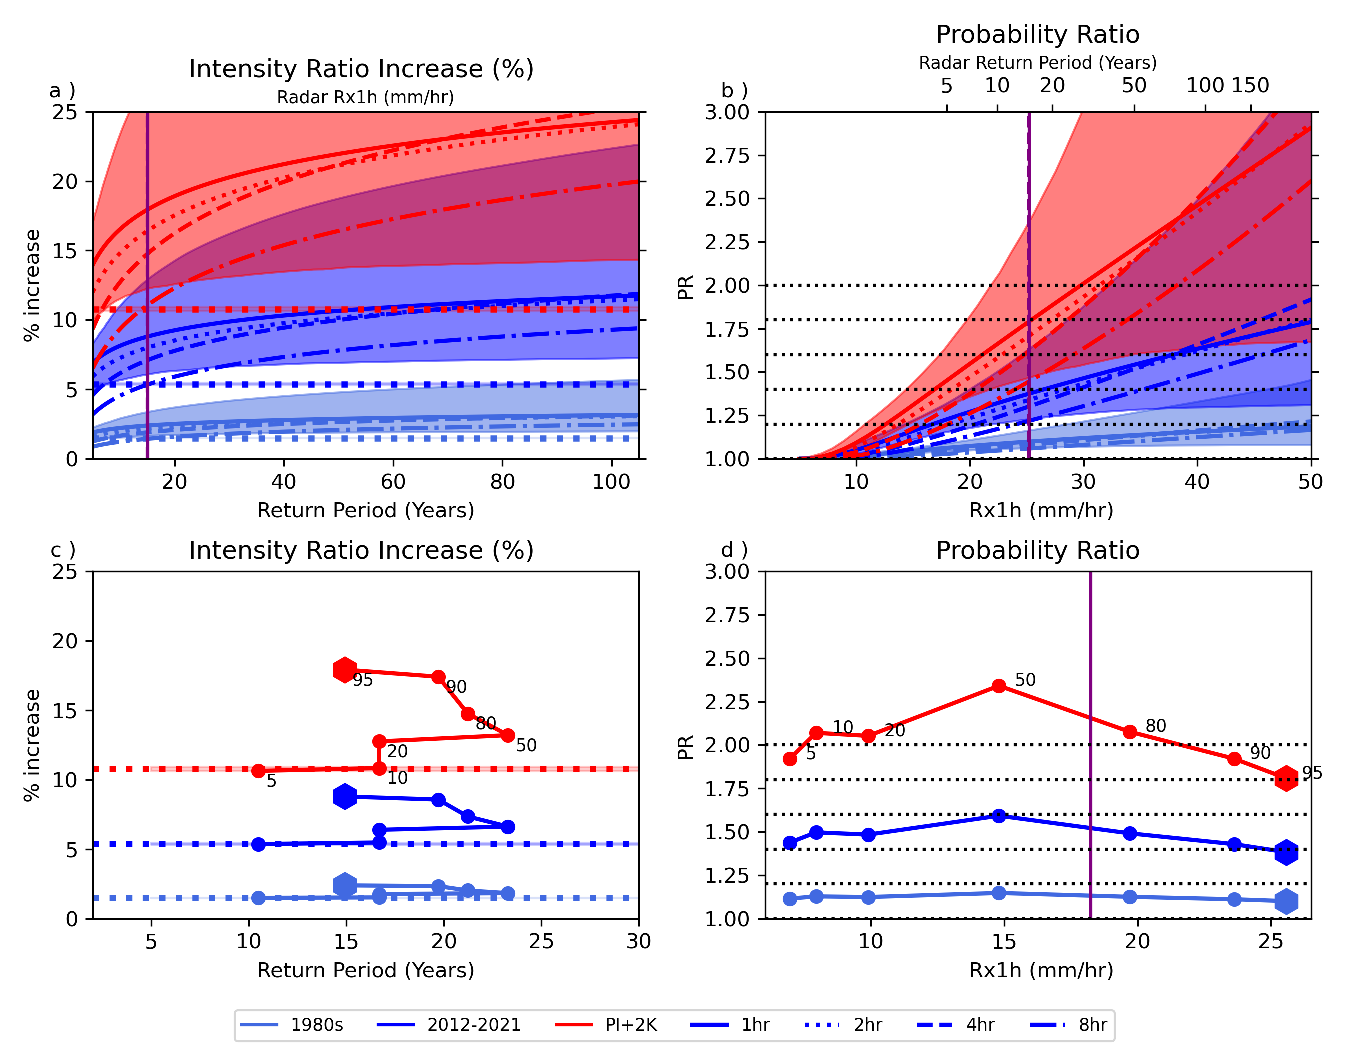
\includegraphics[width=\linewidth]{3probradarcpmshape}
    \end{subfigure}
    \caption[Figures~\ref{fig:2probradarcpm} and~\ref{fig:2probradarcpmshape} for the 2.2km and 6.6km models.]{
        Figure~\ref{fig:2probradarcpm} for the 2.2km model (top left) and the 6.6km model (top right).
    Figure~\ref{fig:2probradarcpmshape} for the 2.2km model (bottom left) and the 6.6km model (bottom right)}
    \label{fig:13probradarcpm}
\end{figure}

One clear difference between the plots in figure~\ref{fig:13probradarcpm} is the finer confidence intervals
    when working with the 2.2km radar data, due to the dataset being larger,
    as well as the very wide confidence intervals for the 6.6km data,
    due to the lack of data giving poor confidence intervals for the model parameter scalings.

For the ratios obtained from both the 2.2km and 6.6km model,
    similar behaviour to that of the 4.4km is found when looking at the effect of using scalings from model rainfall maximum time intervals larger than 1 hour.
As in figures~\ref{fig:2probradarcpm} and~\ref{fig:2probradarcpmshape},
    the probability ratio decreases as the time interval decreases where the scale parameter is fixed,
    while when the scale parameter is fit to CET covariate,
    this only holds up to a point where the relation inverts.
This inversion point seems to be approximately one in 25 year or 35mm/hr events,
    although this does not apply to the 8 hour time interval for the 6.6km fit.

\begin{table}[H]
   \centering
    \begin{tabular}{c c c c c}
        Time Period & IR (2.2km) (\%) & 5--95\% CI (\%) & IR (6.6km) (\%) & 5--95\% CI (\%) \\
        1980s & 2 & 2--3 & 2 & 1--3 \\
        2012--2021 & 8 & 7--9 & 8 & 5--9 \\
        PI+2K & 17 & 15--19 & 15 & 11--18 \\
        With varying shape: &&&& \\
        1980s & 2 & 2--3 & 2 & 2--3 \\
        2012--2021 & 9 & 7--9 & 9 & 6--13 \\
        PI+2K & 16 & 14--18 & 18 & 12--28 \\
    \end{tabular}
    \caption[Table~\ref{tab:irtable} fot 2.2km and 6.6km resolution model fits.]{
        A table with the intensity ratios $I_1/I_0$ for three different time periods,
        both with and without a covariate shape parameter,
        for the 2.2km and 6.6km resolution model fits.
    $I_1$ is the intensity of the event in the Time Period.
    $I_0$ is the intensity of the event Pre-Industrial (1850-1899).}
    \label{tab:13irtable}
\end{table}

\begin{table}[H]
   \centering
    \begin{tabular}{c c c c c}
        Time Period & PR (2.2km) & 5--95\% CI (\%) & PR (6.6km) & 5--95\% CI \\
        1980s & 1.09 & 1.06--1.14 & 1.08 & 1.05--1.13 \\
        2012--2021 & 1.34 & 1.24--1.55 & 1.31 & 1.19--1.52 \\
        PI+2K & 1.74 & 1.50--2.24 & 1.65 & 1.40--2.16 \\
        With varying shape: &&&& \\
        1980s & 1.09 & 1.06--1.14 & 1.10 & 1.06--1.16 \\
        2012--2021 & 1.33 & 1.23--1.55 & 1.37 & 1.23--1.63 \\
        PI+2K & 1.71 & 1.47--2.22 & 1.79 & 1.47--2.36 \\
    \end{tabular}
    \caption[Table~\ref{tab:prtable} for the 2.2km and 6.6km resolution model fits.]{
        A table with the probability ratios $p_1/p_0$ with confidence intervals for three different time periods,
        both with and without a covariate shape parameter.
    $p_1$ is the probability of the event in the Time Period.
    $p_0$ is the probability of the event Pre-Industrial (1850-1899).}
    \label{tab:13prtable}
\end{table}

For the 6.6km resolution data,
    without the shape fit to the covariate,
    the probability ratios suggest that the 4.4km ratios may be an overestimate.
However,
    the ratios match to the nearest hundredth when the shape parameter is considered as a covariate.
As the probability ratios with and without the shape covariate fit are identical for the 4.4km data,
    this suggests that fitting the shape as to the CET covariate may be capturing effects lost from the lower resolution,
    although of the 6.6km fits have an AIC of 6591, suggesting that it is not likely that any information is lost.
Furthermore, for the 6.6km fit with the shape fit to the covariate,
    the intensity ratios decrease if a quantile lower than 0.95 is chosen to give the intensity of an event.

The intensity and probability ratios from the 2.2km and 6.6km model data in tables~\ref{tab:13irtable} and~\ref{tab:13prtable},
    do not differ significantly from those found from the 4.4km model data in tables~\ref{tab:irtable} and~\ref{tab:prtable},
    as the 4.4km ratios lie in the confidence intervals of both of the alternative models and vice versa.
It can then be concluded that changing the model resolution for gathering the parameter scalings does not have a significant effect
     on the outcomes of the event attribution process.

It would not be expected for this analysis to match the disparity in extreme events found by Kendon, Fischer and Short~\cite{Kendon_Fischer_Short_2023}.
This is as the analysis here applies the parameter scaling from different model resolutions to an already fit empirical distribution,
    while the analysis in~\cite{Kendon_Fischer_Short_2023} measures the probability of the model data crossing a threshold.

The model data resolutions providing similar results suggests that the factors driving the change in the maxima are similar between resolutions.

\subsection{Choices in analysis}\label{subsec:diseventdef}

The analysis in subsection~\ref{subsec:dismodeldef} shows that the choice of a 4.4km model resolution over a finer or coarser resolution
    did not have a significant impact on the results.
However,
    many other choices were made in the analysis.
It is necessary to show that these choices do not have a significant effect on the final outcome for the results to be robust.
Where the choices were found to potentially be impactful,
    it is also useful to state whether a more valid choice would suggest that the results are conservative or overstate the impacts.

\subsubsection{Event Definition}

\begin{itemize} \item Stonehaven Region and height mask \end{itemize}

Defining the Stonehaven Region as a 100km$\times$100km square centered on the crash location was deemed valid,
    as choosing a region based on different factors could potentially lead to bias.
The 0m to 400m height mask was considered a valid choice,
    as the catchment of the drain causing the Stonehaven crash peaked at around 200m,
    making 200m the median point of the rainfall.

Figure~\ref{fig:2cpm_gev_fit} (a) and (b) shows that rainfall is much higher in the 200m--400m height range,
    than in the 0m--200m height range,
    with figure~\ref{fig:2cpm_gev_fit} (c) showing that the parameters of the distribution scale more at higher grid cells.
This suggests that the results would understate the risk ratios had a height mask with a lower cap been used.
However, any lower cap would not properly reflect the risk ratios at the Stonehaven crash location,
    as so many points in the 0m--200m height range display far lower rainfall extremes than at Stonehaven.

One additional factor to consider is the homogeneity of the climate of the region used for the analysis.
Looking at the K\"oppen classifications of the Stonehaven Region, given in~\cite{Koppen_file} from WorldClim data~\cite{worldclim},
    the Stonehaven crash location lies on the boundary of Cfb Oceanic and Cfc Subpolar Oceanic.
The defining difference between these definitions is average temperature,
    so it is valid to include both.
The height mask avoids the areas classed as Dfc Subarctic and ET Tundra in the Cairngorms National Park being included in the region.

\begin{itemize}\item Time interval of event\end{itemize}

Although, as can be seen from figure~\ref{fig:stonehavendayraingraph},
    the extreme rainfall at Stonehaven was spread over a four-hour period,
    the event was defined by seasonal one-hour maxima,
    primarily for practical reasons involving the processing of the data.
As this analysis was not done,
    the effect of different time intervals in the definition will be discussed when looking at the effect of
    different time intervals in the model.

\begin{itemize}\item 12-hour bin for event definition\end{itemize}

Each event is defined as occurring within a 12-hour window.
The primary reason for this is to preserve statistical independence,
    as if the seasonal maxima of each grid cell was considered as an extreme rainfall event
    the events may not be independent,
    as extreme rainfall at two locations caused by a single storm would not be independent.

One concern with this approach is that a single storm may pass through the Stonehaven Region
    across two consecutive 12-hour time periods,
    giving two events that are not independent as they describe the same storm.
After applying the minimum size fiter discussed in the next bullet point,
    this occurs for 8 of the 77 events,
    which is unlikely to have a significant effect on the validity GEV fit.

The technique used for the fitting of distributions to the model data,
    where each grid cell has a separate distribution fit to the seasonal maxima,
    clearly maintains statistical independence as each maximum occurs in a different year.
This is not possible for the empirical fit as there are only 18 years of seasonal maxima per grid cell,
    as opposed to the 1200 years simulated in the model,
    and 18 points is insufficient to fit GEV distributions with meaningfully without excessively wide confidence intervals.

\begin{itemize}\item Spatial size of event\end{itemize}

\begin{figure}[H]
    \centering
    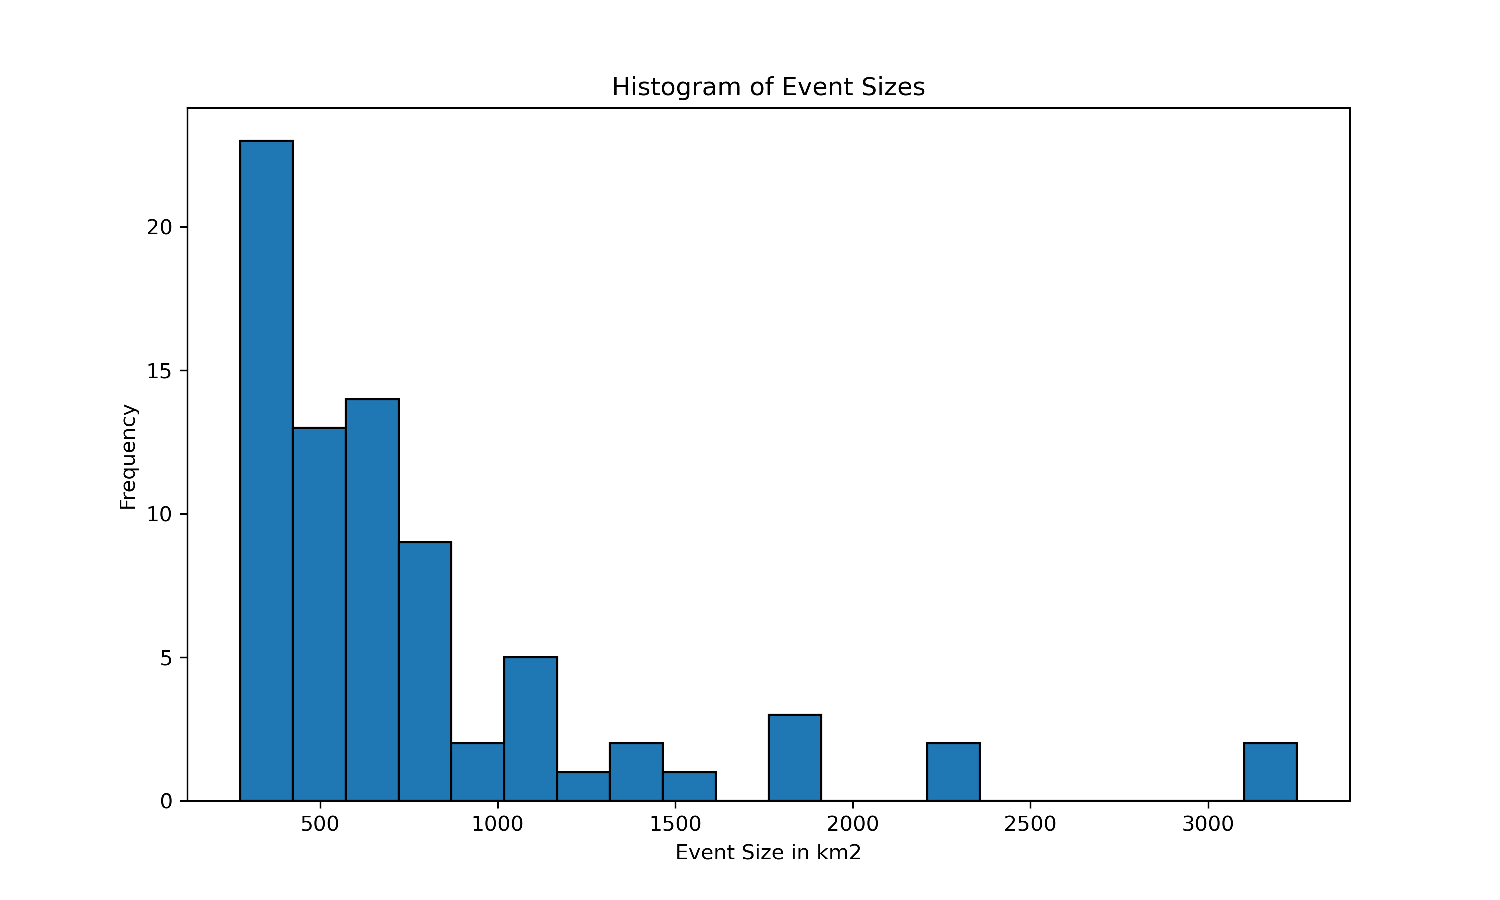
\includegraphics[width=150mm]{eventsizehist}
    \caption[Histogram showing the distribution of event sizes.]{
        Histogram showing the distribution of event sizes in $\text{km}^2$ of the 77 events used the to fit the radar data.
    The Stonehaven Event had a size of 3250$\text{km}^2$,
        being the event covering the largest amount of space.
    No events lower than 250 $\text{km}^2$ are in this histogram as those were removed.}
    \label{fig:eventsizehist}
\end{figure}

Applying the event size filter left only 77 events, as opposed to the 362 separate 12-hour periods in which at least one grid cell had a summer maximum precipitation.
Removing these events was necessary choice as a single cell reaching a maximum does not represent a summer convective storm similar to that causing the Stonehaven Crash.

However,
    it is clear that there are many events which cover a far smaller area of the Stonehaven Region which are being used in the analysis.
There is only one event covering a similar area,
    occurring on the morning of the 28th July 2021.
It is interesting that these events both occurred extremely late in the dataset,
    but a sample size of 2 is insufficient to draw any conclusions about the likelihood of these events changing over time or with changes in temperature.

The Stonehaven Event and the 2021 event covered 127 and 130 of the 185 grid cells respectively,
    leaving 2020 and 2021 to have only 1 and 2 events from other grid cells each.
If this is a strong effect on later years,
    then the empirical fit will be biased to earlier years due to all events being weighted equally.
From figure~\ref{fig:eventsyear}, it can be seen that there is no significant correlation between the
    year and the number of events, so the fit is accurate to the entire time period.

Figure~\ref{fig:eventsyear} provides further evidence that the choice of event size
    was acceptable,
    with the events including the largest 2--7 storms in the region in each year.
When a cutoff greater than 250$\text{km}^2$ was imposed,
    one example of which was 500$\text{km}^2$,
    it was possible to find a GEV fit for the whole dataset.
However,
    the Monte Carlo procedure for estimating confidence intervals resulted in many fits
    to random samples with replacement giving significantly anomalous distributions,
    leading to an overall infinite confidence interval.
Figure~\ref{fig:cellsyear} shows the number of cells contributing to events for a given year.
For all years, the majority of the 185 cells are providing data to the fit.

\begin{figure}[H]
    \centering
    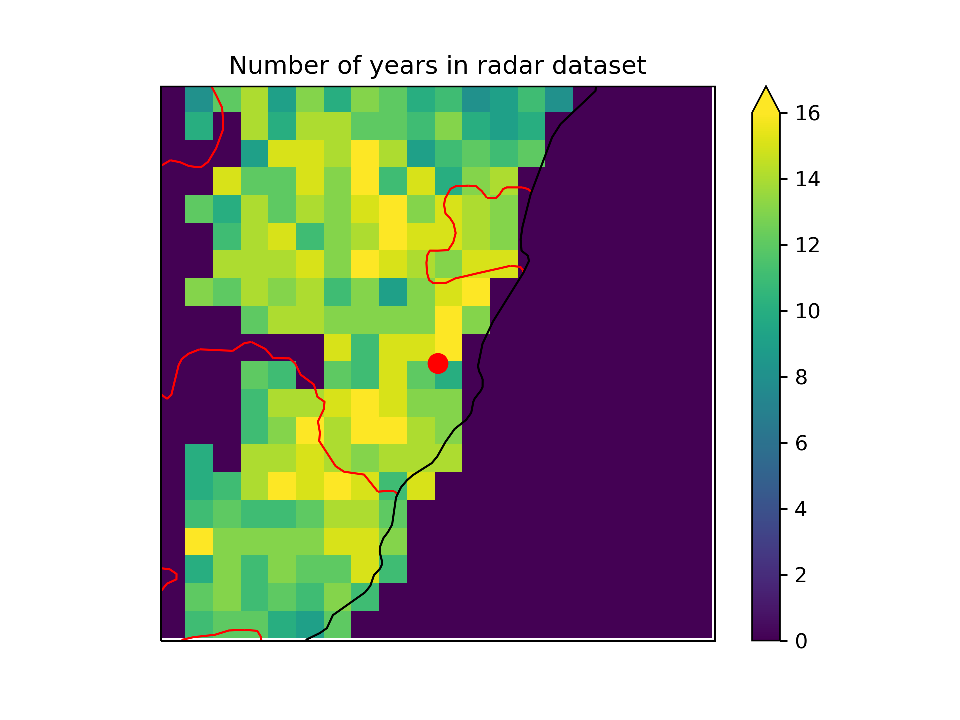
\includegraphics[width=120mm]{yearsinradardata}
    \caption[Plot of the number of years each grid cell appears in an event.]{
        Plot of the number of years each grid cell appears in an event.
    Cells covered by the height mask in figure~\ref{fig:stonetopogallowed}
        do not provide any data.
    Black lines are coastlines, red lines are local authority boundaries.
    Red dot is the crash location.}
    \label{fig:yearsinradardata}
\end{figure}

Comparing the number of times grid cells provide seasonal rainfall maxima to the set of events
    in figure~\ref{fig:yearsinradardata} to the topography in figure~\ref{fig:stonetopog},
    no clear relationship between the topography of the point and the frequency of its appearance in events.
This may suggest that there is no bias towards higher or lower points in the radar data fit.
However,
    as the fit is made to an upper quantile (0.95) of the maximum rainfall at the points contributing to an event,
    this does not directly imply that the fit will not be biased.
For example, if the highest points provide maxima that are in the top quantiles of the event,
    these will have a larger impact on the magnitude used to define the event.

On the other hand,
    by comparing figure~\ref{fig:yearsinradardata} with figure~\ref{fig:stoneregionrain},
    it is seen that the locations of Stonehaven Event are represented disproportionately in the
    locations used to draw the sample of events.
This suggests that the results are more specific to the Stonehaven Event than to other extreme rainfall in the region.
It is unsurprising that the grid cells nearer the centre of the region appear in more events,
    as grid cells nearer to the boundary are more likely to take their summer rainfall maxima
    as a part of a storm that passes near to the Stonehaven Region but is not sufficiently close to
    result in 10 cells taking a maximum value and qualifying as an event.

\begin{itemize}\item Quantile used for intensity of event\end{itemize}

As noted in the discussion of figure~\ref{fig:2probradarcpm},
    the rainfall at the location of the Stonehaven Crash was between the 0.5 and 0.8 quantiles of the Stonehaven Event,
    and the Stonehaven Event was especially unique with the 0.5 and 0.8 quantiles having larger return periods.
This suggests that one of these quantiles may be a more appropriate definition of the intensity of an event,
    as opposed to the 0.95 quantile used for the analysis.

Figure~\ref{fig:2probradarcpm} (c) shows that the intensity ratio is not significantly changed by a choice of parameters,
    suggesting that the intensity ratios found here are robust,
    while (d) shows that the probability ratio is lower for the 0.95 quantile used in the analysis than either of the alternative quantiles,
    suggesting that the probability ratios found here are conservative,
    underestimating the effect of Anthropogenic Climate Change.
As figures~\ref{fig:2probradarcpmshape} and~\ref{fig:13probradarcpm}
    also exhibit this behaviour,
    both of these findings are themselves robust relative to a change in model resolution or a CET scaling of the shape parameter.

The choice of the 0.95 quantile in the original analysis was valid as this is a `more extreme' quantile and was thought to best capture the event's
    effects on the region, as opposed to at the crash location.
The trend in probability ratios continuing for all 4 of the quantiles $\geq$ 0.5 shows that an actual effect is occurring,
    as opposed to an artefact of the 0.95 quantile potentially being ill-defined for small events where fewer than 20 grid cells take seasonal maxima.

\subsubsection{Model Fit}
\begin{itemize}\item Use of different definition from radar data\end{itemize}

As noted in the discussion of 12-hour bins,
    the fit to the model is taken to be the average over the parameters for each grid cell,
    as opposed to the fit to the empirical data being to events as defined above.
For the application of the scaling from the model to be valid,
     it is necessary to justify that the parameters of the event distribution should scale with
    the average parameters of seasonal maximum rainfall of a grid cell in the model.

Each event intensity is,
    by taking a 0.95 quantile,
    effectively a median average over the set of grid cells with seasonal maximum rainfall in the top decile of an event.
It is clear that this would result in both parameters being larger compared to a distribution of seasonal maxima at a single cell,
    as the cells with the largest maximum rainfall are taken to define the distribution.
This is not a concern,
    as the parameter scalings are multiplicative and so proportional to the size of the parameter being scaled,
    seen in equation~\ref{eq:newradarparams}.

However,
    it is uncertain whether this would result in a change in variability between the distributions.
As the event intensity is,
    an effective average over the maximum of multiple grid cells,
    this suggests that there would be less variability as the grid cells with higher and lower summer rainfall maxima will offset one another.
On the other hand,
    taking the grid cells for this median average are always taken from the top decile suggests
    that variability would be increased, as they are in the tail of the distribution where variability is greater
    due to the lower probability density.
The fact that the grid cells of each event differ also suggests that variability would be higher,
    as the maximums are being sampled from different distributions,
    although this would be offset by the rainfall at each point not being independent due to occuring in the same event.
Taking an upper quantile is more valid than taking a mean average of the maximum rainfall in the event,
    as it balances the effects on variability described here.

Consider a simpler event definition of an event being the maximum summer rainfall at a location,
    with a GEV fit made to each location, as for the model data.
If the variability for the definition used in the analysis of this project is greater,
    then the location parameter for the empirical fit is likely an underestimate and the scale parameter is likely
    an overestimate relative to the simpler definition,
    as the scale parameter gives the PDF a wider spread to increase the variability.
This would suggest that the intensity ratios are an overestimate for the simpler definition,
    as the scale parameter scales by a greater amount than the location parameter with CET,
    seen in table~\ref{tab:CCtable},
    and \textit{vice versa} for a lower variability.
It is unclear how this would affect the probability ratios,
    as the underlying distribution would have changed.

It is of note that the hypothetical in the previous paragraph is not desirable,
    as this definition would cover events that are not convective storms,
    being too loose for the Stonehaven Event.
Although the variability concerns should be considered,
    I do not consider these likely to have a large effect on the final result.
This is as both the model and the empirical events are composed of one-hour rainfall maxima driven by the same effects,
    and so would be expected to scale by the same amount with CET .
Testing this hypothesis is beyond the scope of this report.

\begin{itemize}\item Shape parameter fit to covariate\end{itemize}

All the results in subsections~\ref{subsec:covfit} and~\ref{subsec:riskratios} were computed with and without
    the shape parameter $\xi$ fit to the CET covariate.
No significant difference in the results were found,
    showing that the results are robust with respect to this choice.

I do not believe that fitting the shape parameter to the CET covariate would be an appropriate choice to make in this analysis.
Looking at equation~\ref{eq:gevreturn},
    scaling the location $\mu$ and the scale $\sigma$ parameters by the same factor scales the whole distribution,
    including the mean, median and variance.
Scaling both by different factors is also valid,
    as the location parameter scaling will capture a change of the whole distribution,
    while the scale parameter scaling will capture a change that increases as the rarity of the event increases.

There is no similar reason to apply a multiplicative scaling,
    as done by equation~\ref{eq:newradarparams} to the shape parameter.
For small $\xi$, this will have little difference to scaling the shape parameter by the reciprocal factor,
    while, due to the appearance in an exponential,
    there is no reason to expect a simple linear change with the covariate.

This may also lead to clearly incorrect outcomes.
For example, take a model fit with positive shape that finds that the thickness of the tail,
    and so the shape parameter,
    increases with CET,
    but an empirical fit with negative shape, i.e. $\xi_1, \xi_0 > 0$, $\xi_1 / \xi_0 > 1$, $\xi < 0$.
Applying equation~\ref{eq:newradarparams} results in the shape parameter decreasing with CET,
    resulting in the empirical fit becoming more bounded,
    the opposite of that observed in the model.

It is of note that the documentation of the `fevd' command in the extRemes R package states
    that it is ``ill-advised'' to fit the shape parameter to a covariate.

\begin{itemize}\item Time interval of maxima\end{itemize}

As only the one-hour summer rainfall maxima were processed in the radar data to be processed to events for the empirical fit,
    only the one-hour event data was used to directly calculate risk ratios.
However,
    as can be seen in figure~\ref{fig:stonehavendayraingraph},
    the rainfall at Stonehaven was across a 4-hour period,
    which suggests that a 4-hour event definition would be more appropriate.

It is impossible to calculate the exact risk ratios had this alternative definition been used,
    as the exact empirical distribution of these events is not known.
However, the results that are available could suggest what these results may be.

Using an event definition over a longer time period would have meant using scalings from model maxima over that same longer time period.
From table~\ref{tab:CCtable},
    the parameters will then increase by a lesser proportion than was found for the one-hour event definition.
This will likely result in a decreased intensity ratio,
    as the critical value for all probabilities will have increased by a lesser proportion than for the shorter time periods with greater scalings,
    which is visible in figure~\ref{fig:2probradarcpm} (a),
    with the scaling being sub-Clausius-Clapeyron when applying an 8-hour model scaling to the 1-hour empirical fit.
It is also likely that the probability ratios will be lower,
    with the effect being visible in~\ref{fig:2probradarcpm} (b).

As the scalings are decreased,
    the distribution will be increased by a lesser amount and so it is expected that the effect of increased temperature on the return period would be weaker.
This effect is likely to be mitigated by the fact that the Stonehaven event occurred over 4 hours,
    and so is more likely to be rarer and further into the tail of the distribution of 4-hour events,
    where the scale parameter,
    which, from table~\ref{tab:CCtable}, scales more than the location parameter,
    has a more significant effect.
Table one of the RAIB report on the derailment~\cite{RAIB_2022} finds that defining Stonehaven as a three-hour event gives a
    return period of 100 years and a return period of 30 years for a one-hour event,
    in contrast to the 17--24 year return period found here with a one-hour event definition,
    depending on the quantile of the event chosen.

I do not expect this to be near sufficient to undo the effects of the decreased scalings.
Therefore,
    the intensity and probability ratios in this report can be considered overestimates compared to those that would be
    gathered from defining the Stonehaven Event to be over a longer duration.

\subsubsection{Potential future work}

In this analysis,
    it was shown that the maximum summer hourly rainfall distribution had a better fit with the temperature in the Stonehaven Region
    as a covariate than to CET (see table~\ref{tab:AICtable}).
Furthermore,
    whilst the correlation of the Stonehaven Region temperature was reasonably strong ($R^2 = 0.94$),
    the rate of change in temperature in this region did not match with the change in CET (see figure~\ref{fig:2cet_scatter}).
However,
    all the analysis performed here was performed by treating CET as a covariate,
    not the Stonehaven Region temperature,
    with distributions for each time period based on CET in the time period.

The 2K warmer world CET projection directly used that from~\cite{Tett_Soon},
    which was found using a correlation between a processing of a 1961--1990 global surface temperature dataset and CET .
It would be desirable to find the same correlations for the Stonehaven Region temperature,
    but this cannot be done directly as the two nearest weather stations to the Stonehaven Crash location
    with data from this time period~\cite{Old_Stations} are Braemar,
    which has a significantly different climate,
    and Luchars, which is over 70km away.
An additional challenge with this approach is that the data for Pre-Industrial teperatures would also have
    to be extrapolated, as opposed to read directly like CET .

One change that would be straightforward to make would be to find the risk ratios
    using an event intensity defined by the quantile that the Stonehaven Crash rainfall was within the Stonehaven Event.
For reasons given above, the probability ratio would be expected to be greater,
    although the Monte Carlo techniques would also need to be repeated to get a confidence interval for these results.

To get results for longer time intervals,
    such as the four-hour desired for the event in this case,
    the radar data needs to be re-processed.
This would require taking rolling averages,
    as opposed to block averages,
    as is done with the model data,
    to give sufficient data points to describe the longer time periods.

The event definition could also be changed significantly.
For example,
    as opposed to using the AM and PM of a single day to split up events,
    a state of low rain in the region could be used as a boundary,
    separating out events that are known to be independent storms as opposed to using a time cutoff,
    removing the issues with statistical independence in this analysis.

Furthermore,
    this approach could then record the magnitude of the event using all the cells experiencing rainfall above a threshold,
    allowing each grid cell to provide more than the single seasonal maximum data point in a year.
This could then use a Generalised Pareto Distribution~\cite{Coles_2001} instead of the GEV distribution to fit to the data.
To ensure that the region is fairly represented,
    events covering grid cells that have fewer events could be given additional weight in the fit
The event definition could then also be to the model data,
    avoiding the variability concerns as the same definition would be used between both fits.

Whilst the reasons for the shape parameter scaling used in this report being inappropriate are given above,
    that does not mean that the shape parameter must remain fixed.
By replacing the multiplicative scaling in equation~\ref{eq:newradarparams} with an additive scaling of
    $\xi_T = \xi + \delta T \xi_1$,
    the absurd example given is not possible,
    allowing the change in shape parameter to potentially be informative.

One concern not considered in this report is the fact that the model may not be able to represent storms like those of the Stonehaven Event.
A continuation of the work here should then attempt to evaluate this.
One approach would be to look at the model data directly and
    search for events similar to Stonehaven Event and ensure that they match the qualitative features,
    such as the evolution in figure~\ref{fig:stoneregionrain}.
Another would be to enforce the Event Definition onto the model data and check that the parameters of the best fit distributions are similar.

The model evaluation step is particularly challenging in this scenario.
This is as the radar data is only available for 18 years,
    making a trend analysis impossible as any change in the events will not be noticeable
    in comparison to natural variability.
The lack of comparable events in the empirical data makes it very hard to determine the features to use to determine whether a modelled event is comparable.

The analysis here uses the intensity of the extreme rainfall Stonehaven Event itself as a threshold for the analysis,
    so the results in this report therefore do not give the probability ratio for the derailment itself.
For this to be possible,
    hydrological modelling of the flows necessary to cause the debris washout could be performed,
    finding the rainfall threshold at which the event occurs.
Using this threshold,
    probability ratios for the Stonehaven Derailment could be found,
    although these would not account for additional factors,
    such as the landslip causing the reversal in direction.

\subsection{Implications}\label{subsec:disfield}

The approach used in this report has resulted in several points that may be notable for future event attribution studies.

First is the aforementioned effect that the model data had a better fit to temperatures in the region of the event.
This highlights the fact that consideration must be given as to how temperatures in a given region will
    change with Anthropogenic Climate Change when performing an event attribution on the region,
    as opposed to fixing a correlation to a proxy for global temperature.

Second is the sub-Clausius-Clapeyron scaling for the model's summer 8-hour maxima.
As mentioned, this result does not align with the IPCC's~\cite{IPCC_2021}
    expectation of sub-daily rainfall maxima scaling at a rate between in line with and double
    Clausius-Clapeyron.
The reduced scaling gives an increase in extreme precipitation by only 2\% in the bulk
    and 5\% in the tail of the distribution per degree of warming.
Tett et al.~\cite{Tett_Soon} find sub-Clausius-Clapeyron scaling for some grid points in the model,
    but suggest that this effect may be due to a reduction in total rainfall in the region,
    which is also observed in this case, in figure~\ref{fig:2cet_scatter}.

Finally, as per subsection~\ref{subsec:dismodeldef},
    the choice of model resolution used to find scalings with respect to temperature change
    had no significant effect on the final results.
This suggests that the model resolution may not be a significant consideration,
    so long as the model is used to find scalings to apply to an empirical fit,
    not to exhibit the extreme events themselves.
Extrapolating this to~\cite{Tett_Soon} would suggest that the assumption that the
    scaling of the 2.2km model data with CET is acceptable to apply to the 1km model data and supports the validity of the results regarding the Edinburgh cloud-burst event.